\documentclass[twoside]{book}

% Packages required by doxygen
\usepackage{fixltx2e}
\usepackage{calc}
\usepackage{doxygen}
\usepackage[export]{adjustbox} % also loads graphicx
\usepackage{graphicx}
\usepackage[utf8]{inputenc}
\usepackage{makeidx}
\usepackage{multicol}
\usepackage{multirow}
\PassOptionsToPackage{warn}{textcomp}
\usepackage{textcomp}
\usepackage[nointegrals]{wasysym}
\usepackage[table]{xcolor}

% Font selection
\usepackage[T1]{fontenc}
\usepackage[scaled=.90]{helvet}
\usepackage{courier}
\usepackage{amssymb}
\usepackage{sectsty}
\renewcommand{\familydefault}{\sfdefault}
\allsectionsfont{%
  \fontseries{bc}\selectfont%
  \color{darkgray}%
}
\renewcommand{\DoxyLabelFont}{%
  \fontseries{bc}\selectfont%
  \color{darkgray}%
}
\newcommand{\+}{\discretionary{\mbox{\scriptsize$\hookleftarrow$}}{}{}}

% Page & text layout
\usepackage{geometry}
\geometry{%
  a4paper,%
  top=2.5cm,%
  bottom=2.5cm,%
  left=2.5cm,%
  right=2.5cm%
}
\tolerance=750
\hfuzz=15pt
\hbadness=750
\setlength{\emergencystretch}{15pt}
\setlength{\parindent}{0cm}
\setlength{\parskip}{3ex plus 2ex minus 2ex}
\makeatletter
\renewcommand{\paragraph}{%
  \@startsection{paragraph}{4}{0ex}{-1.0ex}{1.0ex}{%
    \normalfont\normalsize\bfseries\SS@parafont%
  }%
}
\renewcommand{\subparagraph}{%
  \@startsection{subparagraph}{5}{0ex}{-1.0ex}{1.0ex}{%
    \normalfont\normalsize\bfseries\SS@subparafont%
  }%
}
\makeatother

% Headers & footers
\usepackage{fancyhdr}
\pagestyle{fancyplain}
\fancyhead[LE]{\fancyplain{}{\bfseries\thepage}}
\fancyhead[CE]{\fancyplain{}{}}
\fancyhead[RE]{\fancyplain{}{\bfseries\leftmark}}
\fancyhead[LO]{\fancyplain{}{\bfseries\rightmark}}
\fancyhead[CO]{\fancyplain{}{}}
\fancyhead[RO]{\fancyplain{}{\bfseries\thepage}}
\fancyfoot[LE]{\fancyplain{}{}}
\fancyfoot[CE]{\fancyplain{}{}}
\fancyfoot[RE]{\fancyplain{}{\bfseries\scriptsize Generated by Doxygen }}
\fancyfoot[LO]{\fancyplain{}{\bfseries\scriptsize Generated by Doxygen }}
\fancyfoot[CO]{\fancyplain{}{}}
\fancyfoot[RO]{\fancyplain{}{}}
\renewcommand{\footrulewidth}{0.4pt}
\renewcommand{\chaptermark}[1]{%
  \markboth{#1}{}%
}
\renewcommand{\sectionmark}[1]{%
  \markright{\thesection\ #1}%
}

% Indices & bibliography
\usepackage{natbib}
\usepackage[titles]{tocloft}
\setcounter{tocdepth}{3}
\setcounter{secnumdepth}{5}
\makeindex

% Hyperlinks (required, but should be loaded last)
\usepackage{ifpdf}
\ifpdf
  \usepackage[pdftex,pagebackref=true]{hyperref}
\else
  \usepackage[ps2pdf,pagebackref=true]{hyperref}
\fi
\hypersetup{%
  colorlinks=true,%
  linkcolor=blue,%
  citecolor=blue,%
  unicode%
}

% Custom commands
\newcommand{\clearemptydoublepage}{%
  \newpage{\pagestyle{empty}\cleardoublepage}%
}

\usepackage{caption}
\captionsetup{labelsep=space,justification=centering,font={bf},singlelinecheck=off,skip=4pt,position=top}

%===== C O N T E N T S =====

\begin{document}

% Titlepage & ToC
\hypersetup{pageanchor=false,
             bookmarksnumbered=true,
             pdfencoding=unicode
            }
\pagenumbering{alph}
\begin{titlepage}
\vspace*{7cm}
\begin{center}%
{\Large Chess }\\
\vspace*{1cm}
{\large Generated by Doxygen 1.8.14}\\
\end{center}
\end{titlepage}
\clearemptydoublepage
\pagenumbering{roman}
\tableofcontents
\clearemptydoublepage
\pagenumbering{arabic}
\hypersetup{pageanchor=true}

%--- Begin generated contents ---
\chapter{Hierarchical Index}
\section{Class Hierarchy}
This inheritance list is sorted roughly, but not completely, alphabetically\+:\begin{DoxyCompactList}
\item \contentsline{section}{Tests.\+Bishop\+Test}{\pageref{class_tests_1_1_bishop_test}}{}
\item \contentsline{section}{gamelogic.\+Board}{\pageref{classgamelogic_1_1_board}}{}
\item \contentsline{section}{Tests.\+Checkmate\+Test}{\pageref{class_tests_1_1_checkmate_test}}{}
\item Exception\begin{DoxyCompactList}
\item \contentsline{section}{Error.\+Invalid\+Exceptions}{\pageref{class_error_1_1_invalid_exceptions}}{}
\end{DoxyCompactList}
\item \contentsline{section}{gamelogic.\+Game}{\pageref{classgamelogic_1_1_game}}{}
\item \contentsline{section}{Tests.\+King\+Test}{\pageref{class_tests_1_1_king_test}}{}
\item \contentsline{section}{Tests.\+Knight\+Test}{\pageref{class_tests_1_1_knight_test}}{}
\item \contentsline{section}{gamelogic.\+Location}{\pageref{classgamelogic_1_1_location}}{}
\item \contentsline{section}{Tests.\+Pawn\+Test}{\pageref{class_tests_1_1_pawn_test}}{}
\item \contentsline{section}{gamelogic.\+Piece}{\pageref{classgamelogic_1_1_piece}}{}
\begin{DoxyCompactList}
\item \contentsline{section}{gamelogic.\+Bishop}{\pageref{classgamelogic_1_1_bishop}}{}
\item \contentsline{section}{gamelogic.\+King}{\pageref{classgamelogic_1_1_king}}{}
\item \contentsline{section}{gamelogic.\+Knight}{\pageref{classgamelogic_1_1_knight}}{}
\item \contentsline{section}{gamelogic.\+Pawn}{\pageref{classgamelogic_1_1_pawn}}{}
\item \contentsline{section}{gamelogic.\+Prince}{\pageref{classgamelogic_1_1_prince}}{}
\item \contentsline{section}{gamelogic.\+Princess}{\pageref{classgamelogic_1_1_princess}}{}
\item \contentsline{section}{gamelogic.\+Queen}{\pageref{classgamelogic_1_1_queen}}{}
\item \contentsline{section}{gamelogic.\+Rook}{\pageref{classgamelogic_1_1_rook}}{}
\end{DoxyCompactList}
\item \contentsline{section}{gamelogic.\+Player}{\pageref{classgamelogic_1_1_player}}{}
\item \contentsline{section}{Tests.\+Princess\+Test}{\pageref{class_tests_1_1_princess_test}}{}
\item \contentsline{section}{Tests.\+Prince\+Test}{\pageref{class_tests_1_1_prince_test}}{}
\item \contentsline{section}{Tests.\+Queen\+Test}{\pageref{class_tests_1_1_queen_test}}{}
\item \contentsline{section}{Tests.\+Rook\+Test}{\pageref{class_tests_1_1_rook_test}}{}
\item \contentsline{section}{gamelogic.\+Start}{\pageref{classgamelogic_1_1_start}}{}
\item \contentsline{section}{Gui.\+Table}{\pageref{class_gui_1_1_table}}{}
\item \contentsline{section}{gamelogic.\+Type}{\pageref{enumgamelogic_1_1_type}}{}
\end{DoxyCompactList}

\chapter{Class Index}
\section{Class List}
Here are the classes, structs, unions and interfaces with brief descriptions\+:\begin{DoxyCompactList}
\item\contentsline{section}{\mbox{\hyperlink{classgamelogic_1_1_bishop}{gamelogic.\+Bishop}} }{\pageref{classgamelogic_1_1_bishop}}{}
\item\contentsline{section}{\mbox{\hyperlink{class_tests_1_1_bishop_test}{Tests.\+Bishop\+Test}} }{\pageref{class_tests_1_1_bishop_test}}{}
\item\contentsline{section}{\mbox{\hyperlink{classgamelogic_1_1_board}{gamelogic.\+Board}} }{\pageref{classgamelogic_1_1_board}}{}
\item\contentsline{section}{\mbox{\hyperlink{class_tests_1_1_checkmate_test}{Tests.\+Checkmate\+Test}} }{\pageref{class_tests_1_1_checkmate_test}}{}
\item\contentsline{section}{\mbox{\hyperlink{classgamelogic_1_1_game}{gamelogic.\+Game}} }{\pageref{classgamelogic_1_1_game}}{}
\item\contentsline{section}{\mbox{\hyperlink{class_error_1_1_invalid_exceptions}{Error.\+Invalid\+Exceptions}} }{\pageref{class_error_1_1_invalid_exceptions}}{}
\item\contentsline{section}{\mbox{\hyperlink{classgamelogic_1_1_king}{gamelogic.\+King}} }{\pageref{classgamelogic_1_1_king}}{}
\item\contentsline{section}{\mbox{\hyperlink{class_tests_1_1_king_test}{Tests.\+King\+Test}} }{\pageref{class_tests_1_1_king_test}}{}
\item\contentsline{section}{\mbox{\hyperlink{classgamelogic_1_1_knight}{gamelogic.\+Knight}} }{\pageref{classgamelogic_1_1_knight}}{}
\item\contentsline{section}{\mbox{\hyperlink{class_tests_1_1_knight_test}{Tests.\+Knight\+Test}} }{\pageref{class_tests_1_1_knight_test}}{}
\item\contentsline{section}{\mbox{\hyperlink{classgamelogic_1_1_location}{gamelogic.\+Location}} }{\pageref{classgamelogic_1_1_location}}{}
\item\contentsline{section}{\mbox{\hyperlink{classgamelogic_1_1_pawn}{gamelogic.\+Pawn}} }{\pageref{classgamelogic_1_1_pawn}}{}
\item\contentsline{section}{\mbox{\hyperlink{class_tests_1_1_pawn_test}{Tests.\+Pawn\+Test}} }{\pageref{class_tests_1_1_pawn_test}}{}
\item\contentsline{section}{\mbox{\hyperlink{classgamelogic_1_1_piece}{gamelogic.\+Piece}} }{\pageref{classgamelogic_1_1_piece}}{}
\item\contentsline{section}{\mbox{\hyperlink{classgamelogic_1_1_player}{gamelogic.\+Player}} }{\pageref{classgamelogic_1_1_player}}{}
\item\contentsline{section}{\mbox{\hyperlink{classgamelogic_1_1_prince}{gamelogic.\+Prince}} }{\pageref{classgamelogic_1_1_prince}}{}
\item\contentsline{section}{\mbox{\hyperlink{classgamelogic_1_1_princess}{gamelogic.\+Princess}} }{\pageref{classgamelogic_1_1_princess}}{}
\item\contentsline{section}{\mbox{\hyperlink{class_tests_1_1_princess_test}{Tests.\+Princess\+Test}} }{\pageref{class_tests_1_1_princess_test}}{}
\item\contentsline{section}{\mbox{\hyperlink{class_tests_1_1_prince_test}{Tests.\+Prince\+Test}} }{\pageref{class_tests_1_1_prince_test}}{}
\item\contentsline{section}{\mbox{\hyperlink{classgamelogic_1_1_queen}{gamelogic.\+Queen}} }{\pageref{classgamelogic_1_1_queen}}{}
\item\contentsline{section}{\mbox{\hyperlink{class_tests_1_1_queen_test}{Tests.\+Queen\+Test}} }{\pageref{class_tests_1_1_queen_test}}{}
\item\contentsline{section}{\mbox{\hyperlink{classgamelogic_1_1_rook}{gamelogic.\+Rook}} }{\pageref{classgamelogic_1_1_rook}}{}
\item\contentsline{section}{\mbox{\hyperlink{class_tests_1_1_rook_test}{Tests.\+Rook\+Test}} }{\pageref{class_tests_1_1_rook_test}}{}
\item\contentsline{section}{\mbox{\hyperlink{classgamelogic_1_1_start}{gamelogic.\+Start}} }{\pageref{classgamelogic_1_1_start}}{}
\item\contentsline{section}{\mbox{\hyperlink{class_gui_1_1_table}{Gui.\+Table}} }{\pageref{class_gui_1_1_table}}{}
\item\contentsline{section}{\mbox{\hyperlink{enumgamelogic_1_1_type}{gamelogic.\+Type}} }{\pageref{enumgamelogic_1_1_type}}{}
\end{DoxyCompactList}

\chapter{Class Documentation}
\hypertarget{classgamelogic_1_1_bishop}{}\section{gamelogic.\+Bishop Class Reference}
\label{classgamelogic_1_1_bishop}\index{gamelogic.\+Bishop@{gamelogic.\+Bishop}}
Inheritance diagram for gamelogic.\+Bishop\+:\begin{figure}[H]
\begin{center}
\leavevmode
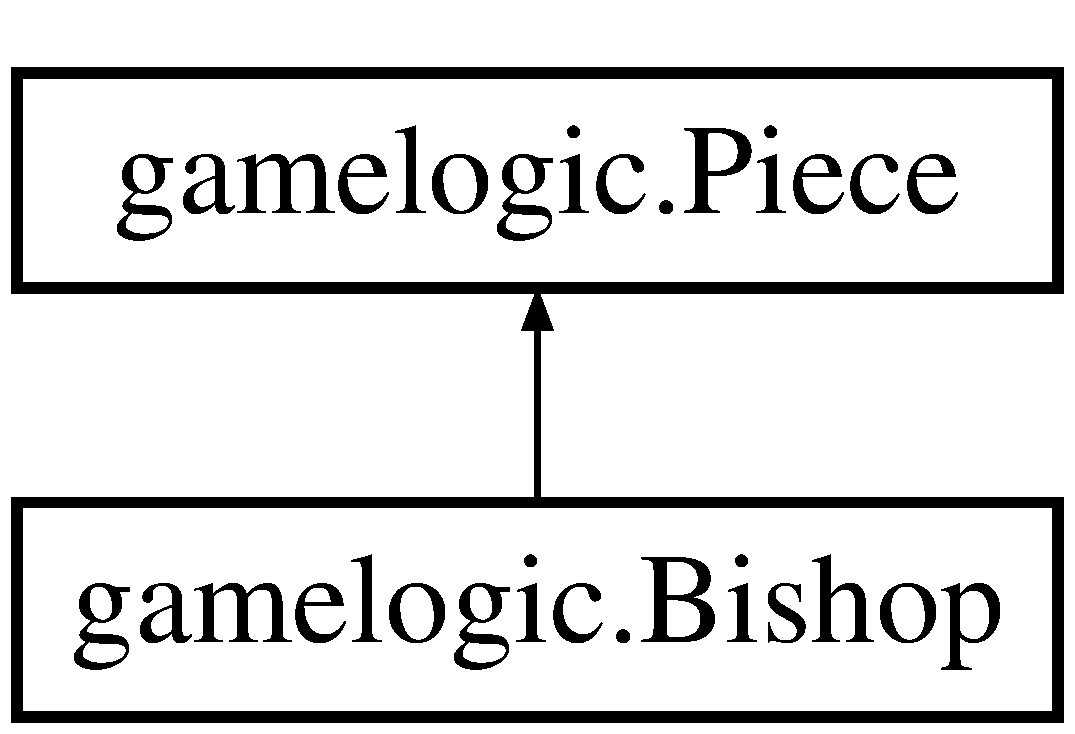
\includegraphics[height=2.000000cm]{classgamelogic_1_1_bishop}
\end{center}
\end{figure}
\subsection*{Public Member Functions}
\begin{DoxyCompactItemize}
\item 
\mbox{\hyperlink{classgamelogic_1_1_bishop_a8012110b6173a72ab217fd1ed14ae71f}{Bishop}} (\mbox{\hyperlink{classgamelogic_1_1_location}{Location}} location, \mbox{\hyperlink{classgamelogic_1_1_player}{Player}} player)
\item 
\mbox{\hyperlink{enumgamelogic_1_1_type}{Type}} \mbox{\hyperlink{classgamelogic_1_1_bishop_a635d8c99a57a092417e0745918217427}{get\+Type}} ()
\item 
boolean \mbox{\hyperlink{classgamelogic_1_1_bishop_a56bffbbf10a9864c982ab2f9142724ce}{legal\+Movement}} (int toI, int toJ, \mbox{\hyperlink{classgamelogic_1_1_start}{Start}} start, \mbox{\hyperlink{classgamelogic_1_1_player}{Player}} player)
\end{DoxyCompactItemize}


\subsection{Constructor \& Destructor Documentation}
\mbox{\Hypertarget{classgamelogic_1_1_bishop_a8012110b6173a72ab217fd1ed14ae71f}\label{classgamelogic_1_1_bishop_a8012110b6173a72ab217fd1ed14ae71f}} 
\index{gamelogic\+::\+Bishop@{gamelogic\+::\+Bishop}!Bishop@{Bishop}}
\index{Bishop@{Bishop}!gamelogic\+::\+Bishop@{gamelogic\+::\+Bishop}}
\subsubsection{\texorpdfstring{Bishop()}{Bishop()}}
{\footnotesize\ttfamily gamelogic.\+Bishop.\+Bishop (\begin{DoxyParamCaption}\item[{\mbox{\hyperlink{classgamelogic_1_1_location}{Location}}}]{location,  }\item[{\mbox{\hyperlink{classgamelogic_1_1_player}{Player}}}]{player }\end{DoxyParamCaption})}

Constructor for \mbox{\hyperlink{classgamelogic_1_1_bishop}{Bishop}}. 
\begin{DoxyParams}{Parameters}
{\em board} & the board object of the current \mbox{\hyperlink{classgamelogic_1_1_board}{Board}} \\
\hline
{\em location} & the location object of the \mbox{\hyperlink{classgamelogic_1_1_board}{Board}} \\
\hline
{\em owner} & the Owner object associated with the \mbox{\hyperlink{classgamelogic_1_1_piece}{Piece}} \\
\hline
\end{DoxyParams}


\subsection{Member Function Documentation}
\mbox{\Hypertarget{classgamelogic_1_1_bishop_a635d8c99a57a092417e0745918217427}\label{classgamelogic_1_1_bishop_a635d8c99a57a092417e0745918217427}} 
\index{gamelogic\+::\+Bishop@{gamelogic\+::\+Bishop}!get\+Type@{get\+Type}}
\index{get\+Type@{get\+Type}!gamelogic\+::\+Bishop@{gamelogic\+::\+Bishop}}
\subsubsection{\texorpdfstring{get\+Type()}{getType()}}
{\footnotesize\ttfamily \mbox{\hyperlink{enumgamelogic_1_1_type}{Type}} gamelogic.\+Bishop.\+get\+Type (\begin{DoxyParamCaption}{ }\end{DoxyParamCaption})}

A function that gets the \mbox{\hyperlink{classgamelogic_1_1_piece}{Piece}} type. \begin{DoxyReturn}{Returns}
an integer indicating the \mbox{\hyperlink{classgamelogic_1_1_piece}{Piece}} type 
\end{DoxyReturn}
\mbox{\Hypertarget{classgamelogic_1_1_bishop_a56bffbbf10a9864c982ab2f9142724ce}\label{classgamelogic_1_1_bishop_a56bffbbf10a9864c982ab2f9142724ce}} 
\index{gamelogic\+::\+Bishop@{gamelogic\+::\+Bishop}!legal\+Movement@{legal\+Movement}}
\index{legal\+Movement@{legal\+Movement}!gamelogic\+::\+Bishop@{gamelogic\+::\+Bishop}}
\subsubsection{\texorpdfstring{legal\+Movement()}{legalMovement()}}
{\footnotesize\ttfamily boolean gamelogic.\+Bishop.\+legal\+Movement (\begin{DoxyParamCaption}\item[{int}]{toI,  }\item[{int}]{toJ,  }\item[{\mbox{\hyperlink{classgamelogic_1_1_start}{Start}}}]{start,  }\item[{\mbox{\hyperlink{classgamelogic_1_1_player}{Player}}}]{player }\end{DoxyParamCaption})}

check Validmove for \mbox{\hyperlink{classgamelogic_1_1_bishop}{Bishop}}. 
\begin{DoxyParams}{Parameters}
{\em x,designated} & row\textquotesingle{}s location \\
\hline
{\em y,designated} & col\textquotesingle{}s location \\
\hline
\end{DoxyParams}
\begin{DoxyReturn}{Returns}
boolean = true if it\textquotesingle{}s valid otherwise false 
\end{DoxyReturn}


The documentation for this class was generated from the following file\+:\begin{DoxyCompactItemize}
\item 
src/gamelogic/Bishop.\+java\end{DoxyCompactItemize}

\hypertarget{class_tests_1_1_bishop_test}{}\section{Tests.\+Bishop\+Test Class Reference}
\label{class_tests_1_1_bishop_test}\index{Tests.\+Bishop\+Test@{Tests.\+Bishop\+Test}}
\subsection*{Public Member Functions}
\begin{DoxyCompactItemize}
\item 
\mbox{\Hypertarget{class_tests_1_1_bishop_test_a1b9cb3227cb0ff2ea8e8b8201db465be}\label{class_tests_1_1_bishop_test_a1b9cb3227cb0ff2ea8e8b8201db465be}} 
void {\bfseries new\+Board} ()  throws Exception
\item 
\mbox{\Hypertarget{class_tests_1_1_bishop_test_a33357092d0ec343da995c66f1f23b3d8}\label{class_tests_1_1_bishop_test_a33357092d0ec343da995c66f1f23b3d8}} 
void {\bfseries valid\+Movements} ()
\item 
\mbox{\Hypertarget{class_tests_1_1_bishop_test_a03f2cbde855c13d3f26437c1fe3f601d}\label{class_tests_1_1_bishop_test_a03f2cbde855c13d3f26437c1fe3f601d}} 
void {\bfseries invalid\+Movements\+Up} ()  throws Exception 
\item 
\mbox{\Hypertarget{class_tests_1_1_bishop_test_aa4b0ab1764449a0d025edd2a6e47152a}\label{class_tests_1_1_bishop_test_aa4b0ab1764449a0d025edd2a6e47152a}} 
void {\bfseries invalid\+Movements\+Down} ()  throws Exception 
\item 
\mbox{\Hypertarget{class_tests_1_1_bishop_test_aac61ed86407ed72f409784fc304b99ef}\label{class_tests_1_1_bishop_test_aac61ed86407ed72f409784fc304b99ef}} 
void {\bfseries invalid\+Movements\+Left} ()  throws Exception 
\item 
\mbox{\Hypertarget{class_tests_1_1_bishop_test_a748c02b9b3fce08a5eb210ef627512ff}\label{class_tests_1_1_bishop_test_a748c02b9b3fce08a5eb210ef627512ff}} 
void {\bfseries invalid\+Movements\+Right} ()  throws Exception 
\item 
\mbox{\Hypertarget{class_tests_1_1_bishop_test_aa79118e5210690e8fbb29e490f355fe5}\label{class_tests_1_1_bishop_test_aa79118e5210690e8fbb29e490f355fe5}} 
void {\bfseries capture} ()  throws Exception 
\end{DoxyCompactItemize}


The documentation for this class was generated from the following file\+:\begin{DoxyCompactItemize}
\item 
src/\+Tests/Bishop\+Test.\+java\end{DoxyCompactItemize}

\hypertarget{classgamelogic_1_1_board}{}\section{gamelogic.\+Board Class Reference}
\label{classgamelogic_1_1_board}\index{gamelogic.\+Board@{gamelogic.\+Board}}
\subsection*{Public Member Functions}
\begin{DoxyCompactItemize}
\item 
\mbox{\hyperlink{classgamelogic_1_1_board_a00654e3d421a89e0532462dc48d85a25}{Board}} ()
\item 
\mbox{\Hypertarget{classgamelogic_1_1_board_a3db0438a1ed6c0bbfd5c35403a4a8a88}\label{classgamelogic_1_1_board_a3db0438a1ed6c0bbfd5c35403a4a8a88}} 
\mbox{\hyperlink{classgamelogic_1_1_piece}{Piece}} \mbox{[}$\,$\mbox{]}\mbox{[}$\,$\mbox{]} {\bfseries get\+Board} ()
\item 
void \mbox{\hyperlink{classgamelogic_1_1_board_a8173f158887a169056c7b1e39cc1885d}{new\+Piece}} (\mbox{\hyperlink{classgamelogic_1_1_piece}{Piece}} piece)
\item 
void \mbox{\hyperlink{classgamelogic_1_1_board_acc3de86741f4e9cec9b31c544937333d}{add\+Piece}} (\mbox{\hyperlink{classgamelogic_1_1_piece}{Piece}} piece, \mbox{\hyperlink{classgamelogic_1_1_location}{Location}} location)
\item 
void \mbox{\hyperlink{classgamelogic_1_1_board_ad538e51550a585d1465d76d92f3ddd10}{remove\+Piece}} (\mbox{\hyperlink{classgamelogic_1_1_piece}{Piece}} piece)
\item 
void \mbox{\hyperlink{classgamelogic_1_1_board_ab7bfac3d534d441e6ebbd1adef05659b}{move\+Piece}} (\mbox{\hyperlink{classgamelogic_1_1_piece}{Piece}} piece, \mbox{\hyperlink{classgamelogic_1_1_location}{Location}} location, \mbox{\hyperlink{classgamelogic_1_1_start}{Start}} start, \mbox{\hyperlink{classgamelogic_1_1_player}{Player}} player)
\item 
\mbox{\hyperlink{classgamelogic_1_1_piece}{Piece}} \mbox{\hyperlink{classgamelogic_1_1_board_ab53a8d50f60e7127e633fd4843e8c20c}{get\+Piece}} (int x, int y)
\item 
\mbox{\Hypertarget{classgamelogic_1_1_board_abc340155b9d2bdb65596446782461e23}\label{classgamelogic_1_1_board_abc340155b9d2bdb65596446782461e23}} 
boolean {\bfseries checked\+Knight} (\mbox{\hyperlink{classgamelogic_1_1_piece}{Piece}} p, \mbox{\hyperlink{classgamelogic_1_1_start}{Start}} start, \mbox{\hyperlink{classgamelogic_1_1_player}{Player}} player)
\item 
\mbox{\Hypertarget{classgamelogic_1_1_board_aec8b979bfaf8320644667436411499d4}\label{classgamelogic_1_1_board_aec8b979bfaf8320644667436411499d4}} 
boolean {\bfseries checked\+Diagonal} (\mbox{\hyperlink{classgamelogic_1_1_piece}{Piece}} p, \mbox{\hyperlink{classgamelogic_1_1_start}{Start}} start, \mbox{\hyperlink{classgamelogic_1_1_player}{Player}} player)
\item 
\mbox{\Hypertarget{classgamelogic_1_1_board_a345735c653c636c63e5d4a1c312ed52e}\label{classgamelogic_1_1_board_a345735c653c636c63e5d4a1c312ed52e}} 
boolean {\bfseries checked\+Straight} (\mbox{\hyperlink{classgamelogic_1_1_piece}{Piece}} piece, \mbox{\hyperlink{classgamelogic_1_1_start}{Start}} start, \mbox{\hyperlink{classgamelogic_1_1_player}{Player}} player)
\item 
\mbox{\Hypertarget{classgamelogic_1_1_board_a8f3209c457b8aac5858e2c4afe3aba40}\label{classgamelogic_1_1_board_a8f3209c457b8aac5858e2c4afe3aba40}} 
boolean {\bfseries ischecked} (\mbox{\hyperlink{classgamelogic_1_1_piece}{Piece}} p, \mbox{\hyperlink{classgamelogic_1_1_start}{Start}} start, \mbox{\hyperlink{classgamelogic_1_1_player}{Player}} player)
\item 
\mbox{\Hypertarget{classgamelogic_1_1_board_aebde91e5d27a19818613c722f3741054}\label{classgamelogic_1_1_board_aebde91e5d27a19818613c722f3741054}} 
boolean {\bfseries is\+Checked\+Mate} (\mbox{\hyperlink{classgamelogic_1_1_piece}{Piece}} p, \mbox{\hyperlink{classgamelogic_1_1_start}{Start}} start, \mbox{\hyperlink{classgamelogic_1_1_player}{Player}} player)
\end{DoxyCompactItemize}


\subsection{Constructor \& Destructor Documentation}
\mbox{\Hypertarget{classgamelogic_1_1_board_a00654e3d421a89e0532462dc48d85a25}\label{classgamelogic_1_1_board_a00654e3d421a89e0532462dc48d85a25}} 
\index{gamelogic\+::\+Board@{gamelogic\+::\+Board}!Board@{Board}}
\index{Board@{Board}!gamelogic\+::\+Board@{gamelogic\+::\+Board}}
\subsubsection{\texorpdfstring{Board()}{Board()}}
{\footnotesize\ttfamily gamelogic.\+Board.\+Board (\begin{DoxyParamCaption}{ }\end{DoxyParamCaption})}

Constructor for the chess board. 
\begin{DoxyParams}{Parameters}
{\em Empty} & create 2D array of size 8x8 \\
\hline
\end{DoxyParams}


\subsection{Member Function Documentation}
\mbox{\Hypertarget{classgamelogic_1_1_board_acc3de86741f4e9cec9b31c544937333d}\label{classgamelogic_1_1_board_acc3de86741f4e9cec9b31c544937333d}} 
\index{gamelogic\+::\+Board@{gamelogic\+::\+Board}!add\+Piece@{add\+Piece}}
\index{add\+Piece@{add\+Piece}!gamelogic\+::\+Board@{gamelogic\+::\+Board}}
\subsubsection{\texorpdfstring{add\+Piece()}{addPiece()}}
{\footnotesize\ttfamily void gamelogic.\+Board.\+add\+Piece (\begin{DoxyParamCaption}\item[{\mbox{\hyperlink{classgamelogic_1_1_piece}{Piece}}}]{piece,  }\item[{\mbox{\hyperlink{classgamelogic_1_1_location}{Location}}}]{location }\end{DoxyParamCaption})}

Function to add piece to current tiles 
\begin{DoxyParams}{Parameters}
{\em \mbox{\hyperlink{classgamelogic_1_1_piece}{Piece}}} & the \mbox{\hyperlink{classgamelogic_1_1_piece}{Piece}} object \\
\hline
{\em \mbox{\hyperlink{classgamelogic_1_1_location}{Location}}} & the location object \\
\hline
\end{DoxyParams}
\mbox{\Hypertarget{classgamelogic_1_1_board_ab53a8d50f60e7127e633fd4843e8c20c}\label{classgamelogic_1_1_board_ab53a8d50f60e7127e633fd4843e8c20c}} 
\index{gamelogic\+::\+Board@{gamelogic\+::\+Board}!get\+Piece@{get\+Piece}}
\index{get\+Piece@{get\+Piece}!gamelogic\+::\+Board@{gamelogic\+::\+Board}}
\subsubsection{\texorpdfstring{get\+Piece()}{getPiece()}}
{\footnotesize\ttfamily \mbox{\hyperlink{classgamelogic_1_1_piece}{Piece}} gamelogic.\+Board.\+get\+Piece (\begin{DoxyParamCaption}\item[{int}]{x,  }\item[{int}]{y }\end{DoxyParamCaption})}

Function from \mbox{\hyperlink{classgamelogic_1_1_piece}{Piece}} class to retrieve the arrays. 
\begin{DoxyParams}{Parameters}
{\em x} & the Row\textquotesingle{}s coordinate \\
\hline
{\em y} & the Col\textquotesingle{}s coordinate \\
\hline
\end{DoxyParams}
\begin{DoxyReturn}{Returns}
the tiles if it\textquotesingle{}s not out-\/of-\/bound 
\end{DoxyReturn}
\mbox{\Hypertarget{classgamelogic_1_1_board_ab7bfac3d534d441e6ebbd1adef05659b}\label{classgamelogic_1_1_board_ab7bfac3d534d441e6ebbd1adef05659b}} 
\index{gamelogic\+::\+Board@{gamelogic\+::\+Board}!move\+Piece@{move\+Piece}}
\index{move\+Piece@{move\+Piece}!gamelogic\+::\+Board@{gamelogic\+::\+Board}}
\subsubsection{\texorpdfstring{move\+Piece()}{movePiece()}}
{\footnotesize\ttfamily void gamelogic.\+Board.\+move\+Piece (\begin{DoxyParamCaption}\item[{\mbox{\hyperlink{classgamelogic_1_1_piece}{Piece}}}]{piece,  }\item[{\mbox{\hyperlink{classgamelogic_1_1_location}{Location}}}]{location,  }\item[{\mbox{\hyperlink{classgamelogic_1_1_start}{Start}}}]{start,  }\item[{\mbox{\hyperlink{classgamelogic_1_1_player}{Player}}}]{player }\end{DoxyParamCaption})}

Function to move piece 
\begin{DoxyParams}{Parameters}
{\em \mbox{\hyperlink{classgamelogic_1_1_piece}{Piece}}} & the \mbox{\hyperlink{classgamelogic_1_1_piece}{Piece}} object \\
\hline
{\em \mbox{\hyperlink{classgamelogic_1_1_location}{Location}}} & the location object \\
\hline
\end{DoxyParams}
\mbox{\Hypertarget{classgamelogic_1_1_board_a8173f158887a169056c7b1e39cc1885d}\label{classgamelogic_1_1_board_a8173f158887a169056c7b1e39cc1885d}} 
\index{gamelogic\+::\+Board@{gamelogic\+::\+Board}!new\+Piece@{new\+Piece}}
\index{new\+Piece@{new\+Piece}!gamelogic\+::\+Board@{gamelogic\+::\+Board}}
\subsubsection{\texorpdfstring{new\+Piece()}{newPiece()}}
{\footnotesize\ttfamily void gamelogic.\+Board.\+new\+Piece (\begin{DoxyParamCaption}\item[{\mbox{\hyperlink{classgamelogic_1_1_piece}{Piece}}}]{piece }\end{DoxyParamCaption})}

function to initialize piece 
\begin{DoxyParams}{Parameters}
{\em \mbox{\hyperlink{classgamelogic_1_1_piece}{Piece}}} & get the piece types \\
\hline
\end{DoxyParams}
\mbox{\Hypertarget{classgamelogic_1_1_board_ad538e51550a585d1465d76d92f3ddd10}\label{classgamelogic_1_1_board_ad538e51550a585d1465d76d92f3ddd10}} 
\index{gamelogic\+::\+Board@{gamelogic\+::\+Board}!remove\+Piece@{remove\+Piece}}
\index{remove\+Piece@{remove\+Piece}!gamelogic\+::\+Board@{gamelogic\+::\+Board}}
\subsubsection{\texorpdfstring{remove\+Piece()}{removePiece()}}
{\footnotesize\ttfamily void gamelogic.\+Board.\+remove\+Piece (\begin{DoxyParamCaption}\item[{\mbox{\hyperlink{classgamelogic_1_1_piece}{Piece}}}]{piece }\end{DoxyParamCaption})}

Function to remove piece add current tiles 
\begin{DoxyParams}{Parameters}
{\em \mbox{\hyperlink{classgamelogic_1_1_piece}{Piece}}} & the \mbox{\hyperlink{classgamelogic_1_1_piece}{Piece}} object \\
\hline
\end{DoxyParams}


The documentation for this class was generated from the following file\+:\begin{DoxyCompactItemize}
\item 
src/gamelogic/Board.\+java\end{DoxyCompactItemize}

\hypertarget{class_tests_1_1_checkmate_test}{}\section{Tests.\+Checkmate\+Test Class Reference}
\label{class_tests_1_1_checkmate_test}\index{Tests.\+Checkmate\+Test@{Tests.\+Checkmate\+Test}}
\subsection*{Public Member Functions}
\begin{DoxyCompactItemize}
\item 
\mbox{\Hypertarget{class_tests_1_1_checkmate_test_adf6782d7c9679ccb7e986c1eb62c205f}\label{class_tests_1_1_checkmate_test_adf6782d7c9679ccb7e986c1eb62c205f}} 
void {\bfseries checkmate} ()
\end{DoxyCompactItemize}


The documentation for this class was generated from the following file\+:\begin{DoxyCompactItemize}
\item 
src/\+Tests/Checkmate\+Test.\+java\end{DoxyCompactItemize}

\hypertarget{classgamelogic_1_1_game}{}\section{gamelogic.\+Game Class Reference}
\label{classgamelogic_1_1_game}\index{gamelogic.\+Game@{gamelogic.\+Game}}
\subsection*{Public Member Functions}
\begin{DoxyCompactItemize}
\item 
\mbox{\Hypertarget{classgamelogic_1_1_game_aeb453c7041c229536de42a1196b2297a}\label{classgamelogic_1_1_game_aeb453c7041c229536de42a1196b2297a}} 
\mbox{\hyperlink{classgamelogic_1_1_piece}{Piece}} {\bfseries get\+Piece} (int i, int j)
\end{DoxyCompactItemize}


The documentation for this class was generated from the following file\+:\begin{DoxyCompactItemize}
\item 
src/gamelogic/Game.\+java\end{DoxyCompactItemize}

\hypertarget{class_error_1_1_invalid_exceptions}{}\section{Error.\+Invalid\+Exceptions Class Reference}
\label{class_error_1_1_invalid_exceptions}\index{Error.\+Invalid\+Exceptions@{Error.\+Invalid\+Exceptions}}
Inheritance diagram for Error.\+Invalid\+Exceptions\+:\begin{figure}[H]
\begin{center}
\leavevmode
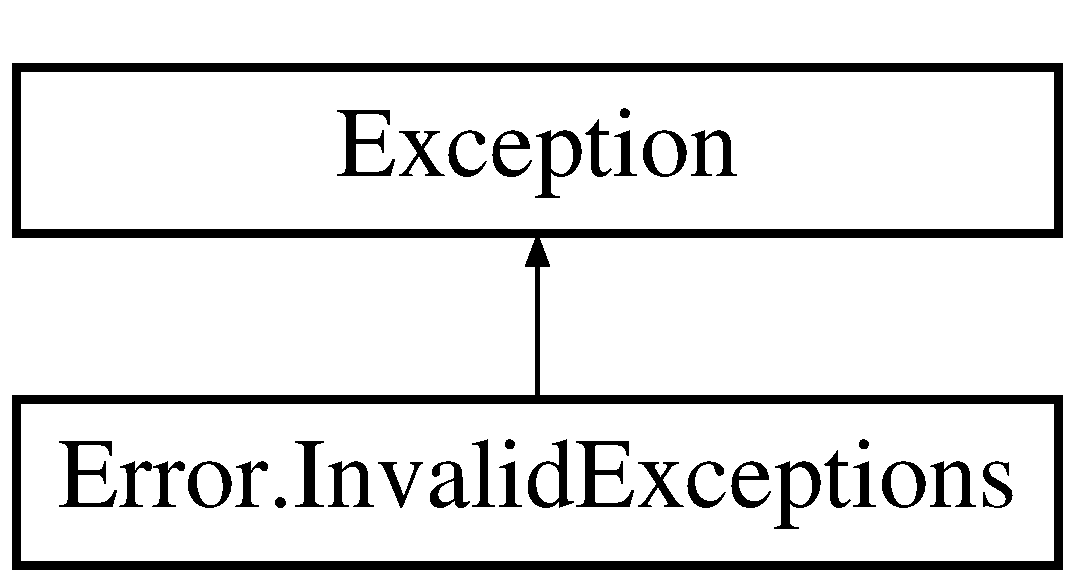
\includegraphics[height=2.000000cm]{class_error_1_1_invalid_exceptions}
\end{center}
\end{figure}


The documentation for this class was generated from the following file\+:\begin{DoxyCompactItemize}
\item 
src/\+Error/Invalid\+Exceptions.\+java\end{DoxyCompactItemize}

\hypertarget{classgamelogic_1_1_king}{}\section{gamelogic.\+King Class Reference}
\label{classgamelogic_1_1_king}\index{gamelogic.\+King@{gamelogic.\+King}}
Inheritance diagram for gamelogic.\+King\+:\begin{figure}[H]
\begin{center}
\leavevmode
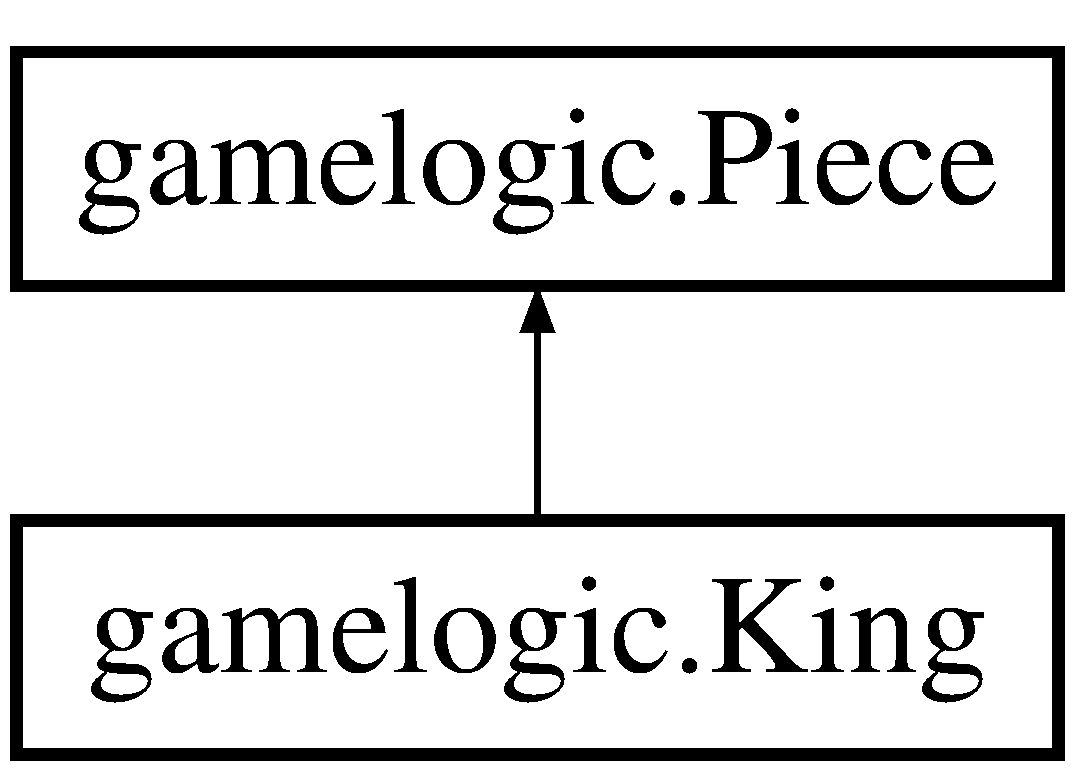
\includegraphics[height=2.000000cm]{classgamelogic_1_1_king}
\end{center}
\end{figure}
\subsection*{Public Member Functions}
\begin{DoxyCompactItemize}
\item 
\mbox{\hyperlink{classgamelogic_1_1_king_a48e0937857b41ac6efc514220c0fdb2b}{King}} (\mbox{\hyperlink{classgamelogic_1_1_location}{Location}} location, \mbox{\hyperlink{classgamelogic_1_1_player}{Player}} player)
\item 
\mbox{\hyperlink{enumgamelogic_1_1_type}{Type}} \mbox{\hyperlink{classgamelogic_1_1_king_a664d6c675ccc53f2eb98bfbfa87eec74}{get\+Type}} ()
\item 
boolean \mbox{\hyperlink{classgamelogic_1_1_king_a4f7b56210475f032b8d6200aa925513a}{legal\+Movement}} (int toI, int toJ, \mbox{\hyperlink{classgamelogic_1_1_start}{Start}} start, \mbox{\hyperlink{classgamelogic_1_1_player}{Player}} player)
\end{DoxyCompactItemize}


\subsection{Constructor \& Destructor Documentation}
\mbox{\Hypertarget{classgamelogic_1_1_king_a48e0937857b41ac6efc514220c0fdb2b}\label{classgamelogic_1_1_king_a48e0937857b41ac6efc514220c0fdb2b}} 
\index{gamelogic\+::\+King@{gamelogic\+::\+King}!King@{King}}
\index{King@{King}!gamelogic\+::\+King@{gamelogic\+::\+King}}
\subsubsection{\texorpdfstring{King()}{King()}}
{\footnotesize\ttfamily gamelogic.\+King.\+King (\begin{DoxyParamCaption}\item[{\mbox{\hyperlink{classgamelogic_1_1_location}{Location}}}]{location,  }\item[{\mbox{\hyperlink{classgamelogic_1_1_player}{Player}}}]{player }\end{DoxyParamCaption})}

Constructor for \mbox{\hyperlink{classgamelogic_1_1_king}{King}}. 
\begin{DoxyParams}{Parameters}
{\em board} & the board object of the current \mbox{\hyperlink{classgamelogic_1_1_board}{Board}} \\
\hline
{\em location} & the location object of the \mbox{\hyperlink{classgamelogic_1_1_board}{Board}} \\
\hline
{\em owner} & the Owner object associated with the \mbox{\hyperlink{classgamelogic_1_1_piece}{Piece}} \\
\hline
\end{DoxyParams}


\subsection{Member Function Documentation}
\mbox{\Hypertarget{classgamelogic_1_1_king_a664d6c675ccc53f2eb98bfbfa87eec74}\label{classgamelogic_1_1_king_a664d6c675ccc53f2eb98bfbfa87eec74}} 
\index{gamelogic\+::\+King@{gamelogic\+::\+King}!get\+Type@{get\+Type}}
\index{get\+Type@{get\+Type}!gamelogic\+::\+King@{gamelogic\+::\+King}}
\subsubsection{\texorpdfstring{get\+Type()}{getType()}}
{\footnotesize\ttfamily \mbox{\hyperlink{enumgamelogic_1_1_type}{Type}} gamelogic.\+King.\+get\+Type (\begin{DoxyParamCaption}{ }\end{DoxyParamCaption})}

A function that gets the \mbox{\hyperlink{classgamelogic_1_1_piece}{Piece}} type. \begin{DoxyReturn}{Returns}
an integer indicating the \mbox{\hyperlink{classgamelogic_1_1_piece}{Piece}} type 
\end{DoxyReturn}
\mbox{\Hypertarget{classgamelogic_1_1_king_a4f7b56210475f032b8d6200aa925513a}\label{classgamelogic_1_1_king_a4f7b56210475f032b8d6200aa925513a}} 
\index{gamelogic\+::\+King@{gamelogic\+::\+King}!legal\+Movement@{legal\+Movement}}
\index{legal\+Movement@{legal\+Movement}!gamelogic\+::\+King@{gamelogic\+::\+King}}
\subsubsection{\texorpdfstring{legal\+Movement()}{legalMovement()}}
{\footnotesize\ttfamily boolean gamelogic.\+King.\+legal\+Movement (\begin{DoxyParamCaption}\item[{int}]{toI,  }\item[{int}]{toJ,  }\item[{\mbox{\hyperlink{classgamelogic_1_1_start}{Start}}}]{start,  }\item[{\mbox{\hyperlink{classgamelogic_1_1_player}{Player}}}]{player }\end{DoxyParamCaption})}

check Validmove for \mbox{\hyperlink{classgamelogic_1_1_king}{King}}. 
\begin{DoxyParams}{Parameters}
{\em toX,designated} & row\textquotesingle{}s location \\
\hline
{\em toY,designated} & col\textquotesingle{}s location \\
\hline
\end{DoxyParams}
\begin{DoxyReturn}{Returns}
boolean = true if it\textquotesingle{}s valid otherwise false 
\end{DoxyReturn}


The documentation for this class was generated from the following file\+:\begin{DoxyCompactItemize}
\item 
src/gamelogic/King.\+java\end{DoxyCompactItemize}

\hypertarget{class_tests_1_1_king_test}{}\section{Tests.\+King\+Test Class Reference}
\label{class_tests_1_1_king_test}\index{Tests.\+King\+Test@{Tests.\+King\+Test}}
\subsection*{Public Member Functions}
\begin{DoxyCompactItemize}
\item 
\mbox{\Hypertarget{class_tests_1_1_king_test_a88b383cdf430afd0b43d98c67594938b}\label{class_tests_1_1_king_test_a88b383cdf430afd0b43d98c67594938b}} 
void {\bfseries new\+Start} ()  throws Exception
\item 
\mbox{\Hypertarget{class_tests_1_1_king_test_af1d0fa8df3379993293e247e99f6fba7}\label{class_tests_1_1_king_test_af1d0fa8df3379993293e247e99f6fba7}} 
void {\bfseries valid\+Movements} ()
\item 
\mbox{\Hypertarget{class_tests_1_1_king_test_abefaadc68b4e1eeada87321158799eb9}\label{class_tests_1_1_king_test_abefaadc68b4e1eeada87321158799eb9}} 
void {\bfseries invalid\+Movements\+More\+Than1} ()  throws Exception 
\item 
\mbox{\Hypertarget{class_tests_1_1_king_test_ae12f7a13c2cb9cd21987e92fe4c364c8}\label{class_tests_1_1_king_test_ae12f7a13c2cb9cd21987e92fe4c364c8}} 
void {\bfseries capture} ()  throws Exception 
\end{DoxyCompactItemize}


The documentation for this class was generated from the following file\+:\begin{DoxyCompactItemize}
\item 
src/\+Tests/King\+Test.\+java\end{DoxyCompactItemize}

\hypertarget{classgamelogic_1_1_knight}{}\section{gamelogic.\+Knight Class Reference}
\label{classgamelogic_1_1_knight}\index{gamelogic.\+Knight@{gamelogic.\+Knight}}
Inheritance diagram for gamelogic.\+Knight\+:\begin{figure}[H]
\begin{center}
\leavevmode
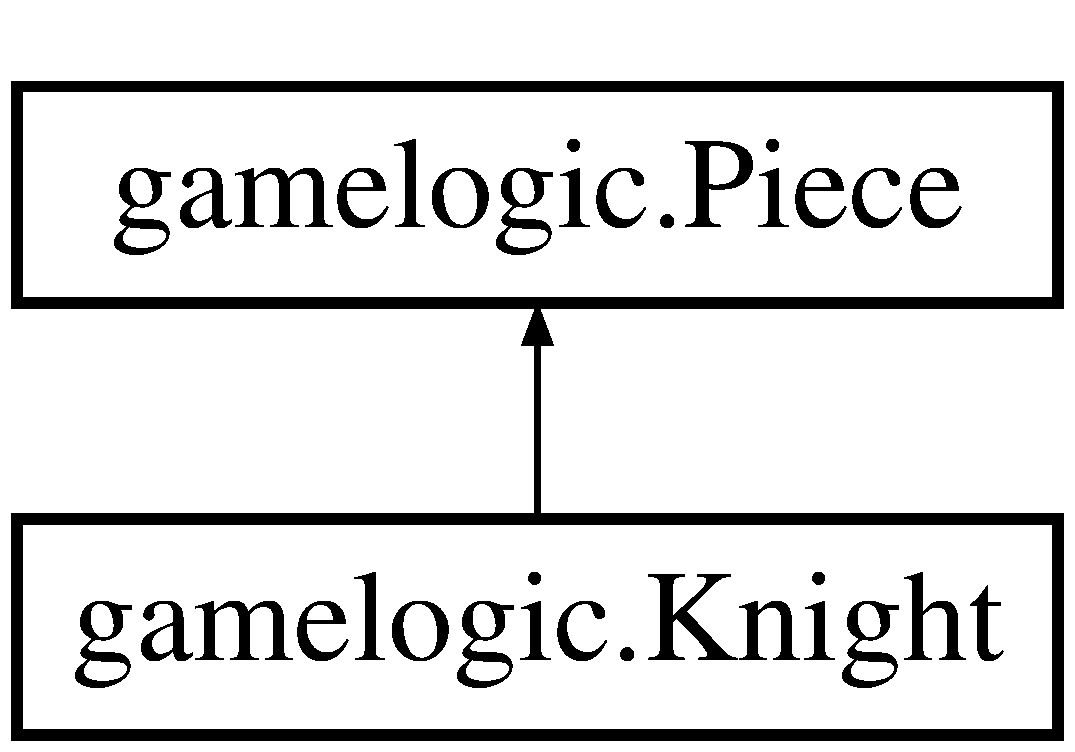
\includegraphics[height=2.000000cm]{classgamelogic_1_1_knight}
\end{center}
\end{figure}
\subsection*{Public Member Functions}
\begin{DoxyCompactItemize}
\item 
\mbox{\hyperlink{classgamelogic_1_1_knight_a149e5fbffb36225d9ef068f6dbd73969}{Knight}} (\mbox{\hyperlink{classgamelogic_1_1_location}{Location}} location, \mbox{\hyperlink{classgamelogic_1_1_player}{Player}} player)
\item 
\mbox{\hyperlink{enumgamelogic_1_1_type}{Type}} \mbox{\hyperlink{classgamelogic_1_1_knight_a4f0d2e001a9cd1c0917677101f794d67}{get\+Type}} ()
\item 
boolean \mbox{\hyperlink{classgamelogic_1_1_knight_a4032e172c78addf1145765a8d53871b9}{legal\+Movement}} (int toI, int toJ, \mbox{\hyperlink{classgamelogic_1_1_start}{Start}} start, \mbox{\hyperlink{classgamelogic_1_1_player}{Player}} player)
\end{DoxyCompactItemize}


\subsection{Constructor \& Destructor Documentation}
\mbox{\Hypertarget{classgamelogic_1_1_knight_a149e5fbffb36225d9ef068f6dbd73969}\label{classgamelogic_1_1_knight_a149e5fbffb36225d9ef068f6dbd73969}} 
\index{gamelogic\+::\+Knight@{gamelogic\+::\+Knight}!Knight@{Knight}}
\index{Knight@{Knight}!gamelogic\+::\+Knight@{gamelogic\+::\+Knight}}
\subsubsection{\texorpdfstring{Knight()}{Knight()}}
{\footnotesize\ttfamily gamelogic.\+Knight.\+Knight (\begin{DoxyParamCaption}\item[{\mbox{\hyperlink{classgamelogic_1_1_location}{Location}}}]{location,  }\item[{\mbox{\hyperlink{classgamelogic_1_1_player}{Player}}}]{player }\end{DoxyParamCaption})}

Constructor for \mbox{\hyperlink{classgamelogic_1_1_knight}{Knight}}. 
\begin{DoxyParams}{Parameters}
{\em board} & the board object of the current \mbox{\hyperlink{classgamelogic_1_1_board}{Board}} \\
\hline
{\em location} & the location object of the \mbox{\hyperlink{classgamelogic_1_1_board}{Board}} \\
\hline
{\em owner} & the Owner object associated with the \mbox{\hyperlink{classgamelogic_1_1_piece}{Piece}} \\
\hline
\end{DoxyParams}


\subsection{Member Function Documentation}
\mbox{\Hypertarget{classgamelogic_1_1_knight_a4f0d2e001a9cd1c0917677101f794d67}\label{classgamelogic_1_1_knight_a4f0d2e001a9cd1c0917677101f794d67}} 
\index{gamelogic\+::\+Knight@{gamelogic\+::\+Knight}!get\+Type@{get\+Type}}
\index{get\+Type@{get\+Type}!gamelogic\+::\+Knight@{gamelogic\+::\+Knight}}
\subsubsection{\texorpdfstring{get\+Type()}{getType()}}
{\footnotesize\ttfamily \mbox{\hyperlink{enumgamelogic_1_1_type}{Type}} gamelogic.\+Knight.\+get\+Type (\begin{DoxyParamCaption}{ }\end{DoxyParamCaption})}

A function that gets the \mbox{\hyperlink{classgamelogic_1_1_piece}{Piece}} type. \begin{DoxyReturn}{Returns}
an integer indicating the \mbox{\hyperlink{classgamelogic_1_1_piece}{Piece}} type 
\end{DoxyReturn}
\mbox{\Hypertarget{classgamelogic_1_1_knight_a4032e172c78addf1145765a8d53871b9}\label{classgamelogic_1_1_knight_a4032e172c78addf1145765a8d53871b9}} 
\index{gamelogic\+::\+Knight@{gamelogic\+::\+Knight}!legal\+Movement@{legal\+Movement}}
\index{legal\+Movement@{legal\+Movement}!gamelogic\+::\+Knight@{gamelogic\+::\+Knight}}
\subsubsection{\texorpdfstring{legal\+Movement()}{legalMovement()}}
{\footnotesize\ttfamily boolean gamelogic.\+Knight.\+legal\+Movement (\begin{DoxyParamCaption}\item[{int}]{toI,  }\item[{int}]{toJ,  }\item[{\mbox{\hyperlink{classgamelogic_1_1_start}{Start}}}]{start,  }\item[{\mbox{\hyperlink{classgamelogic_1_1_player}{Player}}}]{player }\end{DoxyParamCaption})}

check Validmove for \mbox{\hyperlink{classgamelogic_1_1_knight}{Knight}}. 
\begin{DoxyParams}{Parameters}
{\em toX,designated} & row\textquotesingle{}s location \\
\hline
{\em toY,designated} & col\textquotesingle{}s location \\
\hline
\end{DoxyParams}
\begin{DoxyReturn}{Returns}
boolean = true if it\textquotesingle{}s valid otherwise false 
\end{DoxyReturn}


The documentation for this class was generated from the following file\+:\begin{DoxyCompactItemize}
\item 
src/gamelogic/Knight.\+java\end{DoxyCompactItemize}

\hypertarget{class_tests_1_1_knight_test}{}\section{Tests.\+Knight\+Test Class Reference}
\label{class_tests_1_1_knight_test}\index{Tests.\+Knight\+Test@{Tests.\+Knight\+Test}}
\subsection*{Public Member Functions}
\begin{DoxyCompactItemize}
\item 
\mbox{\Hypertarget{class_tests_1_1_knight_test_a062d6fedd7149d5b75682b31cac7789f}\label{class_tests_1_1_knight_test_a062d6fedd7149d5b75682b31cac7789f}} 
void {\bfseries new\+Start} ()  throws Exception
\item 
\mbox{\Hypertarget{class_tests_1_1_knight_test_a7ccc03bd5ca43d8369c65e3ef74da6d4}\label{class_tests_1_1_knight_test_a7ccc03bd5ca43d8369c65e3ef74da6d4}} 
void {\bfseries valid\+Movements\+Bottom\+Left} ()
\item 
\mbox{\Hypertarget{class_tests_1_1_knight_test_a983e3fcdd2c1bf0276a29c8ee34ede50}\label{class_tests_1_1_knight_test_a983e3fcdd2c1bf0276a29c8ee34ede50}} 
void {\bfseries valid\+Movements\+Down\+Left} ()
\item 
\mbox{\Hypertarget{class_tests_1_1_knight_test_a9c9ca411e49f307179bb81aee65db1fa}\label{class_tests_1_1_knight_test_a9c9ca411e49f307179bb81aee65db1fa}} 
void {\bfseries valid\+Movements\+Upper\+Left} ()
\item 
\mbox{\Hypertarget{class_tests_1_1_knight_test_a07459a46da7f61dec19f60da244a83e3}\label{class_tests_1_1_knight_test_a07459a46da7f61dec19f60da244a83e3}} 
void {\bfseries valid\+Movements\+Top\+Left} ()
\item 
\mbox{\Hypertarget{class_tests_1_1_knight_test_ad1f43038c5dbf58e2ce7f6ad5ed6e598}\label{class_tests_1_1_knight_test_ad1f43038c5dbf58e2ce7f6ad5ed6e598}} 
void {\bfseries valid\+Movements\+Top\+Right} ()
\item 
\mbox{\Hypertarget{class_tests_1_1_knight_test_abff93a70489ce212e088244db84f53a0}\label{class_tests_1_1_knight_test_abff93a70489ce212e088244db84f53a0}} 
void {\bfseries valid\+Movements\+Upper\+Right} ()
\item 
\mbox{\Hypertarget{class_tests_1_1_knight_test_a774f32ab19a81a1dd08ee4cdbfc13c04}\label{class_tests_1_1_knight_test_a774f32ab19a81a1dd08ee4cdbfc13c04}} 
void {\bfseries valid\+Movements\+Down\+Right} ()
\item 
\mbox{\Hypertarget{class_tests_1_1_knight_test_a055d87ed6d511ff80c404b7933dc11f4}\label{class_tests_1_1_knight_test_a055d87ed6d511ff80c404b7933dc11f4}} 
void {\bfseries valid\+Movements\+Bottom\+Right} ()
\item 
\mbox{\Hypertarget{class_tests_1_1_knight_test_a82485a7cedb48ae900622c566d7327cc}\label{class_tests_1_1_knight_test_a82485a7cedb48ae900622c566d7327cc}} 
void {\bfseries invalid\+Movements\+Up} ()
\item 
\mbox{\Hypertarget{class_tests_1_1_knight_test_ae43351baa72d32b1e764a1d251622643}\label{class_tests_1_1_knight_test_ae43351baa72d32b1e764a1d251622643}} 
void {\bfseries invalid\+Movements\+Down} ()
\item 
\mbox{\Hypertarget{class_tests_1_1_knight_test_a624326c362ee889e10eac3b885c5a1f9}\label{class_tests_1_1_knight_test_a624326c362ee889e10eac3b885c5a1f9}} 
void {\bfseries invalid\+Movements\+Left} ()
\item 
\mbox{\Hypertarget{class_tests_1_1_knight_test_a8860770b22c5e47d71582b7915b0306a}\label{class_tests_1_1_knight_test_a8860770b22c5e47d71582b7915b0306a}} 
void {\bfseries invalid\+Movements\+Right} ()
\item 
\mbox{\Hypertarget{class_tests_1_1_knight_test_aec4b46ca7b8b017d354cc9931b567ae2}\label{class_tests_1_1_knight_test_aec4b46ca7b8b017d354cc9931b567ae2}} 
void {\bfseries capture} ()  throws Exception 
\end{DoxyCompactItemize}


The documentation for this class was generated from the following file\+:\begin{DoxyCompactItemize}
\item 
src/\+Tests/Knight\+Test.\+java\end{DoxyCompactItemize}

\hypertarget{classgamelogic_1_1_location}{}\section{gamelogic.\+Location Class Reference}
\label{classgamelogic_1_1_location}\index{gamelogic.\+Location@{gamelogic.\+Location}}
\subsection*{Public Member Functions}
\begin{DoxyCompactItemize}
\item 
\mbox{\hyperlink{classgamelogic_1_1_location_ad89bb2c011cbde7816b66ba9aeb08aef}{Location}} (int row, int col)
\item 
int \mbox{\hyperlink{classgamelogic_1_1_location_a2f7ffddb0a19205378c67bc745bedc83}{get\+Row}} ()
\item 
int \mbox{\hyperlink{classgamelogic_1_1_location_aea6fd7274810050fc0d2b46805c85d6f}{get\+Col}} ()
\end{DoxyCompactItemize}


\subsection{Constructor \& Destructor Documentation}
\mbox{\Hypertarget{classgamelogic_1_1_location_ad89bb2c011cbde7816b66ba9aeb08aef}\label{classgamelogic_1_1_location_ad89bb2c011cbde7816b66ba9aeb08aef}} 
\index{gamelogic\+::\+Location@{gamelogic\+::\+Location}!Location@{Location}}
\index{Location@{Location}!gamelogic\+::\+Location@{gamelogic\+::\+Location}}
\subsubsection{\texorpdfstring{Location()}{Location()}}
{\footnotesize\ttfamily gamelogic.\+Location.\+Location (\begin{DoxyParamCaption}\item[{int}]{row,  }\item[{int}]{col }\end{DoxyParamCaption})}

The constructor for class \mbox{\hyperlink{classgamelogic_1_1_location}{Location}} 
\begin{DoxyParams}{Parameters}
{\em x} & the Row\textquotesingle{}s coordinate \\
\hline
{\em y} & the Col\textquotesingle{}s coordinate \\
\hline
\end{DoxyParams}


\subsection{Member Function Documentation}
\mbox{\Hypertarget{classgamelogic_1_1_location_aea6fd7274810050fc0d2b46805c85d6f}\label{classgamelogic_1_1_location_aea6fd7274810050fc0d2b46805c85d6f}} 
\index{gamelogic\+::\+Location@{gamelogic\+::\+Location}!get\+Col@{get\+Col}}
\index{get\+Col@{get\+Col}!gamelogic\+::\+Location@{gamelogic\+::\+Location}}
\subsubsection{\texorpdfstring{get\+Col()}{getCol()}}
{\footnotesize\ttfamily int gamelogic.\+Location.\+get\+Col (\begin{DoxyParamCaption}{ }\end{DoxyParamCaption})}

A function that gets the column \begin{DoxyReturn}{Returns}
an integer of row 
\end{DoxyReturn}
\mbox{\Hypertarget{classgamelogic_1_1_location_a2f7ffddb0a19205378c67bc745bedc83}\label{classgamelogic_1_1_location_a2f7ffddb0a19205378c67bc745bedc83}} 
\index{gamelogic\+::\+Location@{gamelogic\+::\+Location}!get\+Row@{get\+Row}}
\index{get\+Row@{get\+Row}!gamelogic\+::\+Location@{gamelogic\+::\+Location}}
\subsubsection{\texorpdfstring{get\+Row()}{getRow()}}
{\footnotesize\ttfamily int gamelogic.\+Location.\+get\+Row (\begin{DoxyParamCaption}{ }\end{DoxyParamCaption})}

A function that gets the row \begin{DoxyReturn}{Returns}
an integer of row 
\end{DoxyReturn}


The documentation for this class was generated from the following file\+:\begin{DoxyCompactItemize}
\item 
src/gamelogic/Location.\+java\end{DoxyCompactItemize}

\hypertarget{classgamelogic_1_1_pawn}{}\section{gamelogic.\+Pawn Class Reference}
\label{classgamelogic_1_1_pawn}\index{gamelogic.\+Pawn@{gamelogic.\+Pawn}}
Inheritance diagram for gamelogic.\+Pawn\+:\begin{figure}[H]
\begin{center}
\leavevmode
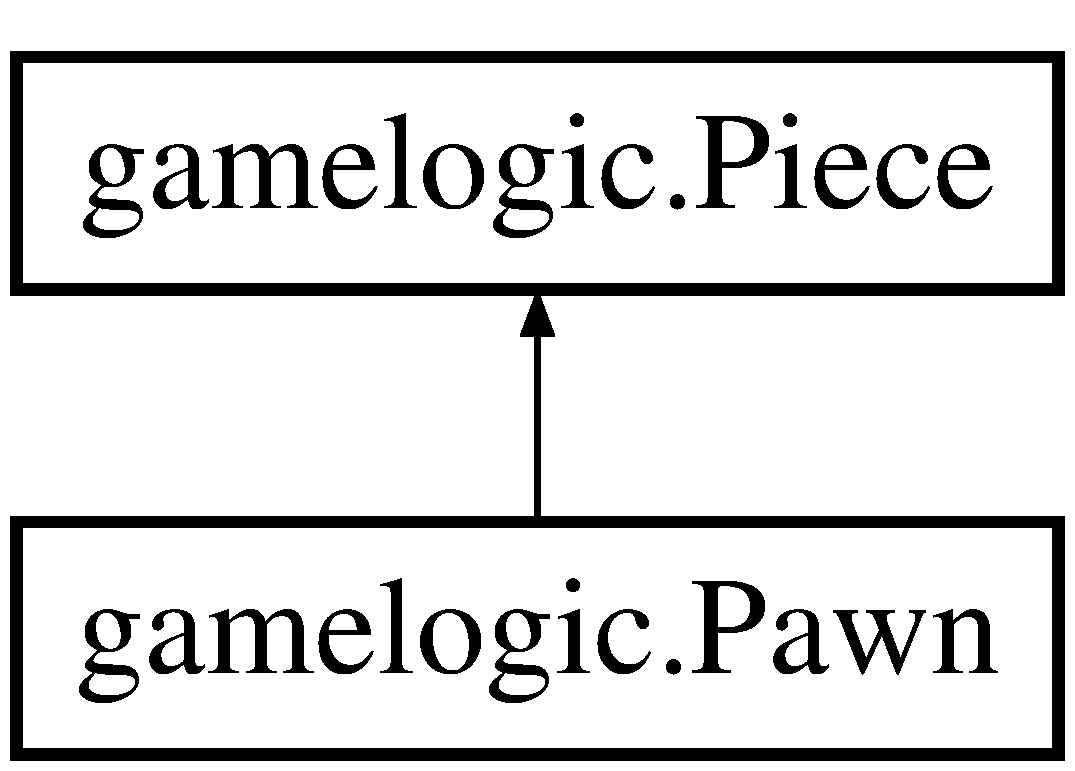
\includegraphics[height=2.000000cm]{classgamelogic_1_1_pawn}
\end{center}
\end{figure}
\subsection*{Public Member Functions}
\begin{DoxyCompactItemize}
\item 
\mbox{\hyperlink{classgamelogic_1_1_pawn_a6ca804bf25a83fe84b36eff001737238}{Pawn}} (\mbox{\hyperlink{classgamelogic_1_1_location}{Location}} location, \mbox{\hyperlink{classgamelogic_1_1_player}{Player}} player)
\item 
\mbox{\hyperlink{enumgamelogic_1_1_type}{Type}} \mbox{\hyperlink{classgamelogic_1_1_pawn_aacb3217a868c5d3dbd98f4f96b6a7c5e}{get\+Type}} ()
\item 
boolean \mbox{\hyperlink{classgamelogic_1_1_pawn_abb8252d13a8a01c9412722543051cf37}{legal\+Movement}} (int toI, int toJ, \mbox{\hyperlink{classgamelogic_1_1_start}{Start}} start, \mbox{\hyperlink{classgamelogic_1_1_player}{Player}} player)
\end{DoxyCompactItemize}


\subsection{Constructor \& Destructor Documentation}
\mbox{\Hypertarget{classgamelogic_1_1_pawn_a6ca804bf25a83fe84b36eff001737238}\label{classgamelogic_1_1_pawn_a6ca804bf25a83fe84b36eff001737238}} 
\index{gamelogic\+::\+Pawn@{gamelogic\+::\+Pawn}!Pawn@{Pawn}}
\index{Pawn@{Pawn}!gamelogic\+::\+Pawn@{gamelogic\+::\+Pawn}}
\subsubsection{\texorpdfstring{Pawn()}{Pawn()}}
{\footnotesize\ttfamily gamelogic.\+Pawn.\+Pawn (\begin{DoxyParamCaption}\item[{\mbox{\hyperlink{classgamelogic_1_1_location}{Location}}}]{location,  }\item[{\mbox{\hyperlink{classgamelogic_1_1_player}{Player}}}]{player }\end{DoxyParamCaption})}

Constructor for \mbox{\hyperlink{classgamelogic_1_1_pawn}{Pawn}}. 
\begin{DoxyParams}{Parameters}
{\em board} & the board object of the current \mbox{\hyperlink{classgamelogic_1_1_board}{Board}} \\
\hline
{\em location} & the location object of the \mbox{\hyperlink{classgamelogic_1_1_board}{Board}} \\
\hline
{\em owner} & the Owner object associated with the \mbox{\hyperlink{classgamelogic_1_1_piece}{Piece}} \\
\hline
\end{DoxyParams}


\subsection{Member Function Documentation}
\mbox{\Hypertarget{classgamelogic_1_1_pawn_aacb3217a868c5d3dbd98f4f96b6a7c5e}\label{classgamelogic_1_1_pawn_aacb3217a868c5d3dbd98f4f96b6a7c5e}} 
\index{gamelogic\+::\+Pawn@{gamelogic\+::\+Pawn}!get\+Type@{get\+Type}}
\index{get\+Type@{get\+Type}!gamelogic\+::\+Pawn@{gamelogic\+::\+Pawn}}
\subsubsection{\texorpdfstring{get\+Type()}{getType()}}
{\footnotesize\ttfamily \mbox{\hyperlink{enumgamelogic_1_1_type}{Type}} gamelogic.\+Pawn.\+get\+Type (\begin{DoxyParamCaption}{ }\end{DoxyParamCaption})}

A function that gets the \mbox{\hyperlink{classgamelogic_1_1_piece}{Piece}} type. \begin{DoxyReturn}{Returns}
an integer indicating the \mbox{\hyperlink{classgamelogic_1_1_piece}{Piece}} type 
\end{DoxyReturn}
\mbox{\Hypertarget{classgamelogic_1_1_pawn_abb8252d13a8a01c9412722543051cf37}\label{classgamelogic_1_1_pawn_abb8252d13a8a01c9412722543051cf37}} 
\index{gamelogic\+::\+Pawn@{gamelogic\+::\+Pawn}!legal\+Movement@{legal\+Movement}}
\index{legal\+Movement@{legal\+Movement}!gamelogic\+::\+Pawn@{gamelogic\+::\+Pawn}}
\subsubsection{\texorpdfstring{legal\+Movement()}{legalMovement()}}
{\footnotesize\ttfamily boolean gamelogic.\+Pawn.\+legal\+Movement (\begin{DoxyParamCaption}\item[{int}]{toI,  }\item[{int}]{toJ,  }\item[{\mbox{\hyperlink{classgamelogic_1_1_start}{Start}}}]{start,  }\item[{\mbox{\hyperlink{classgamelogic_1_1_player}{Player}}}]{player }\end{DoxyParamCaption})}

check Validmove for \mbox{\hyperlink{classgamelogic_1_1_pawn}{Pawn}}. 
\begin{DoxyParams}{Parameters}
{\em toI,designated} & row\textquotesingle{}s location \\
\hline
{\em toJ,designated} & col\textquotesingle{}s location \\
\hline
\end{DoxyParams}
\begin{DoxyReturn}{Returns}
boolean = true if it\textquotesingle{}s valid otherwise false 
\end{DoxyReturn}


The documentation for this class was generated from the following file\+:\begin{DoxyCompactItemize}
\item 
src/gamelogic/Pawn.\+java\end{DoxyCompactItemize}

\hypertarget{class_tests_1_1_pawn_test}{}\section{Tests.\+Pawn\+Test Class Reference}
\label{class_tests_1_1_pawn_test}\index{Tests.\+Pawn\+Test@{Tests.\+Pawn\+Test}}
\subsection*{Public Member Functions}
\begin{DoxyCompactItemize}
\item 
\mbox{\Hypertarget{class_tests_1_1_pawn_test_a8109849a1e688f09410757cdd3b91b61}\label{class_tests_1_1_pawn_test_a8109849a1e688f09410757cdd3b91b61}} 
void {\bfseries new\+Start} ()  throws Exception
\item 
\mbox{\Hypertarget{class_tests_1_1_pawn_test_a1318533de69d55e17ece4a81c16ae328}\label{class_tests_1_1_pawn_test_a1318533de69d55e17ece4a81c16ae328}} 
void {\bfseries valid\+Movements\+Up\+Player} ()
\item 
\mbox{\Hypertarget{class_tests_1_1_pawn_test_a1747639f2fa30b99d2605a1baa394327}\label{class_tests_1_1_pawn_test_a1747639f2fa30b99d2605a1baa394327}} 
void {\bfseries valid\+Movements\+Up2\+Player} ()
\item 
\mbox{\Hypertarget{class_tests_1_1_pawn_test_a3b54ca0d5d5c7b9e532005f3f37233a7}\label{class_tests_1_1_pawn_test_a3b54ca0d5d5c7b9e532005f3f37233a7}} 
void {\bfseries invalid\+Movements\+Up2\+Player} ()
\item 
\mbox{\Hypertarget{class_tests_1_1_pawn_test_a5efb08a6a46fc44d12eec3e6d26921ff}\label{class_tests_1_1_pawn_test_a5efb08a6a46fc44d12eec3e6d26921ff}} 
void {\bfseries valid\+Movements\+Diag\+Player} ()
\item 
\mbox{\Hypertarget{class_tests_1_1_pawn_test_ae382c81c1ff7a613223e4a3578fb2306}\label{class_tests_1_1_pawn_test_ae382c81c1ff7a613223e4a3578fb2306}} 
void {\bfseries invalid\+Movements\+Diag\+Player} ()
\item 
\mbox{\Hypertarget{class_tests_1_1_pawn_test_a0a398b4aeba3ba21b6e4db502f0728f3}\label{class_tests_1_1_pawn_test_a0a398b4aeba3ba21b6e4db502f0728f3}} 
void {\bfseries capture} ()  throws Exception 
\end{DoxyCompactItemize}


The documentation for this class was generated from the following file\+:\begin{DoxyCompactItemize}
\item 
src/\+Tests/Pawn\+Test.\+java\end{DoxyCompactItemize}

\hypertarget{classgamelogic_1_1_piece}{}\section{gamelogic.\+Piece Class Reference}
\label{classgamelogic_1_1_piece}\index{gamelogic.\+Piece@{gamelogic.\+Piece}}
Inheritance diagram for gamelogic.\+Piece\+:\begin{figure}[H]
\begin{center}
\leavevmode
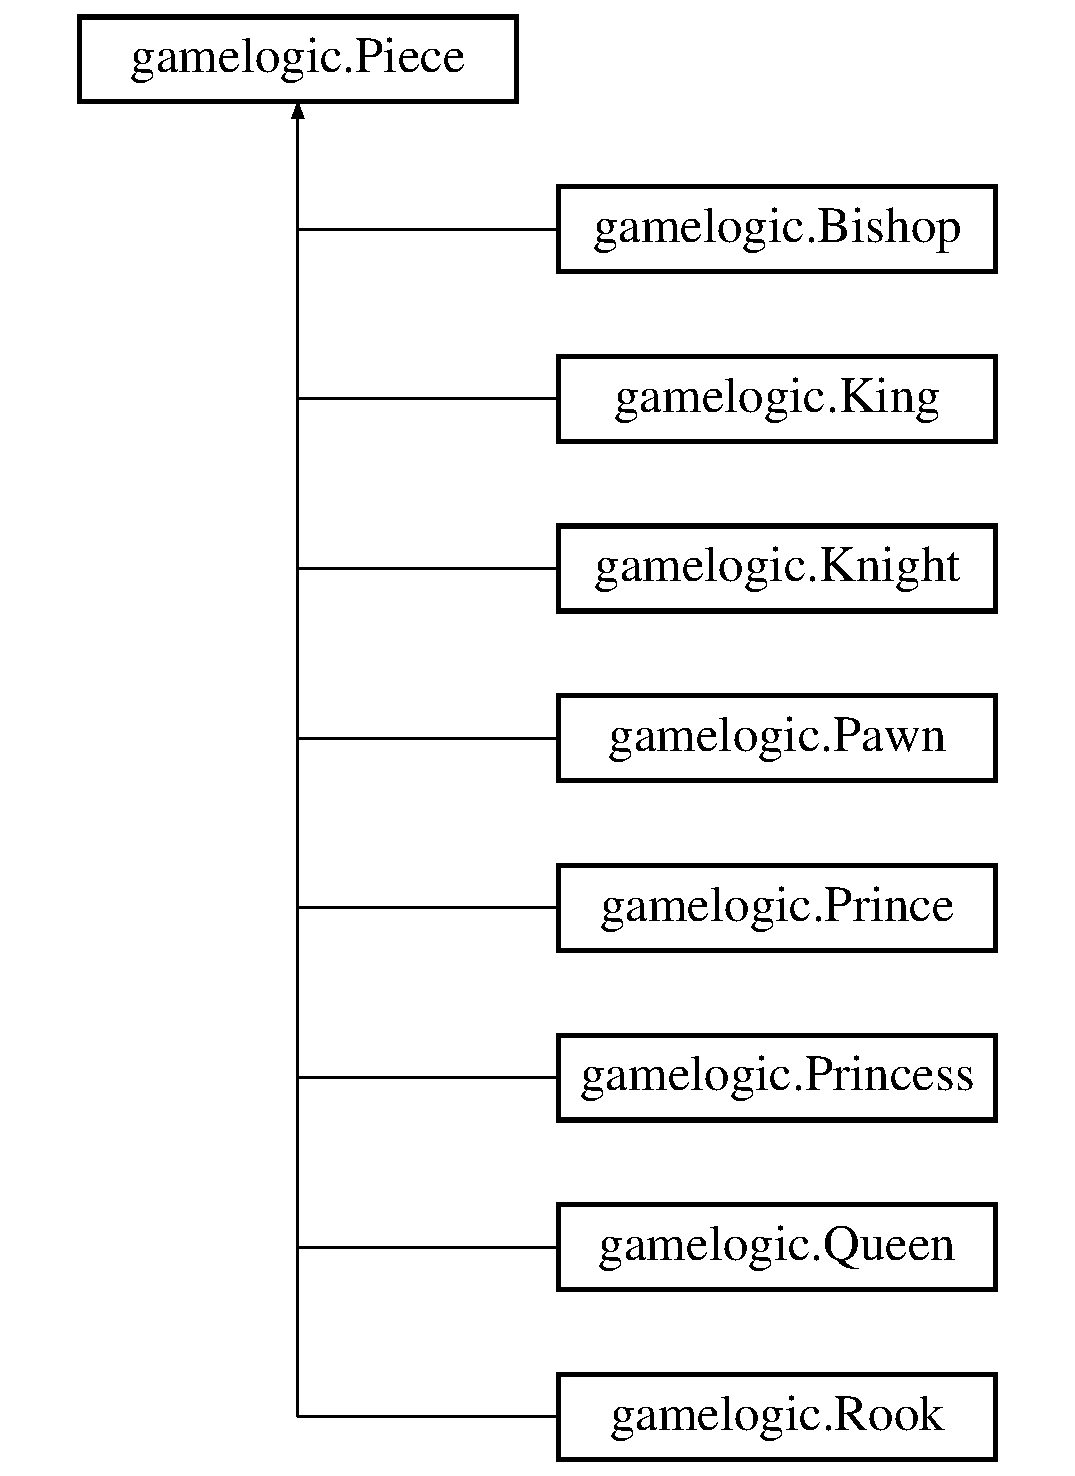
\includegraphics[height=9.000000cm]{classgamelogic_1_1_piece}
\end{center}
\end{figure}
\subsection*{Public Member Functions}
\begin{DoxyCompactItemize}
\item 
\mbox{\hyperlink{classgamelogic_1_1_piece_ab0442f319debc38a447e0e7f7ba3bbf8}{Piece}} (\mbox{\hyperlink{classgamelogic_1_1_location}{Location}} location, \mbox{\hyperlink{classgamelogic_1_1_player}{Player}} player)
\item 
\mbox{\hyperlink{classgamelogic_1_1_location}{Location}} \mbox{\hyperlink{classgamelogic_1_1_piece_a606b1bef122f221d40a88e7b79d54b00}{get\+Location}} ()
\item 
\mbox{\hyperlink{classgamelogic_1_1_player}{Player}} \mbox{\hyperlink{classgamelogic_1_1_piece_a8e8a7aef1b872104c0d6dd6c31474794}{get\+Player}} ()
\item 
\mbox{\Hypertarget{classgamelogic_1_1_piece_af107a61ff3bf8e4641a5bfd0501dbf67}\label{classgamelogic_1_1_piece_af107a61ff3bf8e4641a5bfd0501dbf67}} 
void {\bfseries set\+Location} (\mbox{\hyperlink{classgamelogic_1_1_location}{Location}} location)
\item 
abstract \mbox{\hyperlink{enumgamelogic_1_1_type}{Type}} \mbox{\hyperlink{classgamelogic_1_1_piece_ada7c47c213e0f2271fbab7432cf6de51}{get\+Type}} ()
\item 
abstract boolean \mbox{\hyperlink{classgamelogic_1_1_piece_a443a86d99dabcd09c637cca2344ae3bd}{legal\+Movement}} (int toI, int toJ, \mbox{\hyperlink{classgamelogic_1_1_start}{Start}} start, \mbox{\hyperlink{classgamelogic_1_1_player}{Player}} player)
\item 
\mbox{\Hypertarget{classgamelogic_1_1_piece_ae2db48886123d42187139328c1b0005a}\label{classgamelogic_1_1_piece_ae2db48886123d42187139328c1b0005a}} 
boolean {\bfseries check\+Movement} (int toI, int toJ, \mbox{\hyperlink{classgamelogic_1_1_piece}{Piece}} piece, \mbox{\hyperlink{classgamelogic_1_1_start}{Start}} start, \mbox{\hyperlink{classgamelogic_1_1_player}{Player}} player)
\item 
boolean \mbox{\hyperlink{classgamelogic_1_1_piece_a8a07aab5b997bd7b889e5eb1c72622b0}{is\+Out\+Of\+Bound}} (int i, int j)
\item 
boolean \mbox{\hyperlink{classgamelogic_1_1_piece_a001ebd45357d11f8b742a27b5f358db9}{is\+Path\+Diagonal\+Clear}} (int toI, int toJ, int fromI, int fromJ, \mbox{\hyperlink{classgamelogic_1_1_start}{Start}} start, \mbox{\hyperlink{classgamelogic_1_1_player}{Player}} player)
\item 
boolean \mbox{\hyperlink{classgamelogic_1_1_piece_a3b13e1bdba1f3db5f9e8e5d219599d6c}{is\+Path\+Straight\+Clear}} (int toI, int toJ, int fromI, int fromJ, \mbox{\hyperlink{classgamelogic_1_1_start}{Start}} start, \mbox{\hyperlink{classgamelogic_1_1_player}{Player}} player)
\item 
\mbox{\Hypertarget{classgamelogic_1_1_piece_a4b84a20156cfa3c64362a19150ab35ce}\label{classgamelogic_1_1_piece_a4b84a20156cfa3c64362a19150ab35ce}} 
boolean {\bfseries equals} (\mbox{\hyperlink{classgamelogic_1_1_piece}{Piece}} other)
\end{DoxyCompactItemize}


\subsection{Constructor \& Destructor Documentation}
\mbox{\Hypertarget{classgamelogic_1_1_piece_ab0442f319debc38a447e0e7f7ba3bbf8}\label{classgamelogic_1_1_piece_ab0442f319debc38a447e0e7f7ba3bbf8}} 
\index{gamelogic\+::\+Piece@{gamelogic\+::\+Piece}!Piece@{Piece}}
\index{Piece@{Piece}!gamelogic\+::\+Piece@{gamelogic\+::\+Piece}}
\subsubsection{\texorpdfstring{Piece()}{Piece()}}
{\footnotesize\ttfamily gamelogic.\+Piece.\+Piece (\begin{DoxyParamCaption}\item[{\mbox{\hyperlink{classgamelogic_1_1_location}{Location}}}]{location,  }\item[{\mbox{\hyperlink{classgamelogic_1_1_player}{Player}}}]{player }\end{DoxyParamCaption})}

Constructor for a \mbox{\hyperlink{classgamelogic_1_1_piece}{Piece}}. 
\begin{DoxyParams}{Parameters}
{\em board} & the board object of the \mbox{\hyperlink{classgamelogic_1_1_piece}{Piece}} \\
\hline
{\em location} & the location object of the \mbox{\hyperlink{classgamelogic_1_1_piece}{Piece}} \\
\hline
{\em owner} & the Owner object associated with the \mbox{\hyperlink{classgamelogic_1_1_piece}{Piece}} \\
\hline
\end{DoxyParams}


\subsection{Member Function Documentation}
\mbox{\Hypertarget{classgamelogic_1_1_piece_a606b1bef122f221d40a88e7b79d54b00}\label{classgamelogic_1_1_piece_a606b1bef122f221d40a88e7b79d54b00}} 
\index{gamelogic\+::\+Piece@{gamelogic\+::\+Piece}!get\+Location@{get\+Location}}
\index{get\+Location@{get\+Location}!gamelogic\+::\+Piece@{gamelogic\+::\+Piece}}
\subsubsection{\texorpdfstring{get\+Location()}{getLocation()}}
{\footnotesize\ttfamily \mbox{\hyperlink{classgamelogic_1_1_location}{Location}} gamelogic.\+Piece.\+get\+Location (\begin{DoxyParamCaption}{ }\end{DoxyParamCaption})}

A function getter that gets the location \begin{DoxyReturn}{Returns}
the location object 
\end{DoxyReturn}
\mbox{\Hypertarget{classgamelogic_1_1_piece_a8e8a7aef1b872104c0d6dd6c31474794}\label{classgamelogic_1_1_piece_a8e8a7aef1b872104c0d6dd6c31474794}} 
\index{gamelogic\+::\+Piece@{gamelogic\+::\+Piece}!get\+Player@{get\+Player}}
\index{get\+Player@{get\+Player}!gamelogic\+::\+Piece@{gamelogic\+::\+Piece}}
\subsubsection{\texorpdfstring{get\+Player()}{getPlayer()}}
{\footnotesize\ttfamily \mbox{\hyperlink{classgamelogic_1_1_player}{Player}} gamelogic.\+Piece.\+get\+Player (\begin{DoxyParamCaption}{ }\end{DoxyParamCaption})}

A function getter that gets the player \begin{DoxyReturn}{Returns}
the player object 
\end{DoxyReturn}
\mbox{\Hypertarget{classgamelogic_1_1_piece_ada7c47c213e0f2271fbab7432cf6de51}\label{classgamelogic_1_1_piece_ada7c47c213e0f2271fbab7432cf6de51}} 
\index{gamelogic\+::\+Piece@{gamelogic\+::\+Piece}!get\+Type@{get\+Type}}
\index{get\+Type@{get\+Type}!gamelogic\+::\+Piece@{gamelogic\+::\+Piece}}
\subsubsection{\texorpdfstring{get\+Type()}{getType()}}
{\footnotesize\ttfamily abstract \mbox{\hyperlink{enumgamelogic_1_1_type}{Type}} gamelogic.\+Piece.\+get\+Type (\begin{DoxyParamCaption}{ }\end{DoxyParamCaption})\hspace{0.3cm}{\ttfamily [abstract]}}

An abstract function that returns the type of a \mbox{\hyperlink{classgamelogic_1_1_piece}{Piece}}. \mbox{\Hypertarget{classgamelogic_1_1_piece_a8a07aab5b997bd7b889e5eb1c72622b0}\label{classgamelogic_1_1_piece_a8a07aab5b997bd7b889e5eb1c72622b0}} 
\index{gamelogic\+::\+Piece@{gamelogic\+::\+Piece}!is\+Out\+Of\+Bound@{is\+Out\+Of\+Bound}}
\index{is\+Out\+Of\+Bound@{is\+Out\+Of\+Bound}!gamelogic\+::\+Piece@{gamelogic\+::\+Piece}}
\subsubsection{\texorpdfstring{is\+Out\+Of\+Bound()}{isOutOfBound()}}
{\footnotesize\ttfamily boolean gamelogic.\+Piece.\+is\+Out\+Of\+Bound (\begin{DoxyParamCaption}\item[{int}]{i,  }\item[{int}]{j }\end{DoxyParamCaption})}

Function to check out-\/of-\/boundary. 
\begin{DoxyParams}{Parameters}
{\em i} & the Row\textquotesingle{}s coordinate \\
\hline
{\em j} & the Col\textquotesingle{}s coordinate \\
\hline
\end{DoxyParams}
\begin{DoxyReturn}{Returns}
true if it is out-\/of-\/boundary, otherwise false 
\end{DoxyReturn}
\mbox{\Hypertarget{classgamelogic_1_1_piece_a001ebd45357d11f8b742a27b5f358db9}\label{classgamelogic_1_1_piece_a001ebd45357d11f8b742a27b5f358db9}} 
\index{gamelogic\+::\+Piece@{gamelogic\+::\+Piece}!is\+Path\+Diagonal\+Clear@{is\+Path\+Diagonal\+Clear}}
\index{is\+Path\+Diagonal\+Clear@{is\+Path\+Diagonal\+Clear}!gamelogic\+::\+Piece@{gamelogic\+::\+Piece}}
\subsubsection{\texorpdfstring{is\+Path\+Diagonal\+Clear()}{isPathDiagonalClear()}}
{\footnotesize\ttfamily boolean gamelogic.\+Piece.\+is\+Path\+Diagonal\+Clear (\begin{DoxyParamCaption}\item[{int}]{toI,  }\item[{int}]{toJ,  }\item[{int}]{fromI,  }\item[{int}]{fromJ,  }\item[{\mbox{\hyperlink{classgamelogic_1_1_start}{Start}}}]{start,  }\item[{\mbox{\hyperlink{classgamelogic_1_1_player}{Player}}}]{player }\end{DoxyParamCaption})}

Function to check Diagonal path. 
\begin{DoxyParams}{Parameters}
{\em toI} & the designated X coordinate \\
\hline
{\em toJ} & the designated Y coordinate \\
\hline
{\em fromI} & the current X coordinate \\
\hline
{\em fromJ} & the current Y coordinate \\
\hline
\end{DoxyParams}
\begin{DoxyReturn}{Returns}
true if it is out-\/of-\/boundary, otherwise false 
\end{DoxyReturn}
\mbox{\Hypertarget{classgamelogic_1_1_piece_a3b13e1bdba1f3db5f9e8e5d219599d6c}\label{classgamelogic_1_1_piece_a3b13e1bdba1f3db5f9e8e5d219599d6c}} 
\index{gamelogic\+::\+Piece@{gamelogic\+::\+Piece}!is\+Path\+Straight\+Clear@{is\+Path\+Straight\+Clear}}
\index{is\+Path\+Straight\+Clear@{is\+Path\+Straight\+Clear}!gamelogic\+::\+Piece@{gamelogic\+::\+Piece}}
\subsubsection{\texorpdfstring{is\+Path\+Straight\+Clear()}{isPathStraightClear()}}
{\footnotesize\ttfamily boolean gamelogic.\+Piece.\+is\+Path\+Straight\+Clear (\begin{DoxyParamCaption}\item[{int}]{toI,  }\item[{int}]{toJ,  }\item[{int}]{fromI,  }\item[{int}]{fromJ,  }\item[{\mbox{\hyperlink{classgamelogic_1_1_start}{Start}}}]{start,  }\item[{\mbox{\hyperlink{classgamelogic_1_1_player}{Player}}}]{player }\end{DoxyParamCaption})}

Function to check vertical and horizontal path. 
\begin{DoxyParams}{Parameters}
{\em toI} & the designated X coordinate \\
\hline
{\em toJ} & the designated Y coordinate \\
\hline
{\em fromI} & the current X coordinate \\
\hline
{\em fromJ} & the current Y coordinate \\
\hline
\end{DoxyParams}
\begin{DoxyReturn}{Returns}
true if it is out-\/of-\/boundary, otherwise false 
\end{DoxyReturn}
\mbox{\Hypertarget{classgamelogic_1_1_piece_a443a86d99dabcd09c637cca2344ae3bd}\label{classgamelogic_1_1_piece_a443a86d99dabcd09c637cca2344ae3bd}} 
\index{gamelogic\+::\+Piece@{gamelogic\+::\+Piece}!legal\+Movement@{legal\+Movement}}
\index{legal\+Movement@{legal\+Movement}!gamelogic\+::\+Piece@{gamelogic\+::\+Piece}}
\subsubsection{\texorpdfstring{legal\+Movement()}{legalMovement()}}
{\footnotesize\ttfamily abstract boolean gamelogic.\+Piece.\+legal\+Movement (\begin{DoxyParamCaption}\item[{int}]{toI,  }\item[{int}]{toJ,  }\item[{\mbox{\hyperlink{classgamelogic_1_1_start}{Start}}}]{start,  }\item[{\mbox{\hyperlink{classgamelogic_1_1_player}{Player}}}]{player }\end{DoxyParamCaption})\hspace{0.3cm}{\ttfamily [abstract]}}

Abstract function that is shared among the Pieces type to check if it\textquotesingle{}s a valid move 
\begin{DoxyParams}{Parameters}
{\em toI} & the row\textquotesingle{}s designated location \\
\hline
{\em toJ} & the col\textquotesingle{}s designated location \\
\hline
\end{DoxyParams}
\begin{DoxyReturn}{Returns}
a boolean indicating whether the path is valid 
\end{DoxyReturn}


The documentation for this class was generated from the following file\+:\begin{DoxyCompactItemize}
\item 
src/gamelogic/Piece.\+java\end{DoxyCompactItemize}

\hypertarget{classgamelogic_1_1_player}{}\section{gamelogic.\+Player Class Reference}
\label{classgamelogic_1_1_player}\index{gamelogic.\+Player@{gamelogic.\+Player}}
\subsection*{Public Member Functions}
\begin{DoxyCompactItemize}
\item 
\mbox{\hyperlink{classgamelogic_1_1_player_a1d7ca97131c5bf8912b05aa9475e493f}{Player}} (boolean is\+White)
\item 
boolean \mbox{\hyperlink{classgamelogic_1_1_player_a043caf992b13d5b287c98b0f668b4647}{get\+Player\+Type}} ()
\end{DoxyCompactItemize}


\subsection{Constructor \& Destructor Documentation}
\mbox{\Hypertarget{classgamelogic_1_1_player_a1d7ca97131c5bf8912b05aa9475e493f}\label{classgamelogic_1_1_player_a1d7ca97131c5bf8912b05aa9475e493f}} 
\index{gamelogic\+::\+Player@{gamelogic\+::\+Player}!Player@{Player}}
\index{Player@{Player}!gamelogic\+::\+Player@{gamelogic\+::\+Player}}
\subsubsection{\texorpdfstring{Player()}{Player()}}
{\footnotesize\ttfamily gamelogic.\+Player.\+Player (\begin{DoxyParamCaption}\item[{boolean}]{is\+White }\end{DoxyParamCaption})}

The constructor for class \mbox{\hyperlink{classgamelogic_1_1_location}{Location}} 
\begin{DoxyParams}{Parameters}
{\em x} & the Row\textquotesingle{}s coordinate \\
\hline
{\em y} & the Col\textquotesingle{}s coordinate \\
\hline
\end{DoxyParams}


\subsection{Member Function Documentation}
\mbox{\Hypertarget{classgamelogic_1_1_player_a043caf992b13d5b287c98b0f668b4647}\label{classgamelogic_1_1_player_a043caf992b13d5b287c98b0f668b4647}} 
\index{gamelogic\+::\+Player@{gamelogic\+::\+Player}!get\+Player\+Type@{get\+Player\+Type}}
\index{get\+Player\+Type@{get\+Player\+Type}!gamelogic\+::\+Player@{gamelogic\+::\+Player}}
\subsubsection{\texorpdfstring{get\+Player\+Type()}{getPlayerType()}}
{\footnotesize\ttfamily boolean gamelogic.\+Player.\+get\+Player\+Type (\begin{DoxyParamCaption}{ }\end{DoxyParamCaption})}

A function that gets the boolean \begin{DoxyReturn}{Returns}
true if white, else false. 
\end{DoxyReturn}


The documentation for this class was generated from the following file\+:\begin{DoxyCompactItemize}
\item 
src/gamelogic/Player.\+java\end{DoxyCompactItemize}

\hypertarget{classgamelogic_1_1_prince}{}\section{gamelogic.\+Prince Class Reference}
\label{classgamelogic_1_1_prince}\index{gamelogic.\+Prince@{gamelogic.\+Prince}}
Inheritance diagram for gamelogic.\+Prince\+:\begin{figure}[H]
\begin{center}
\leavevmode
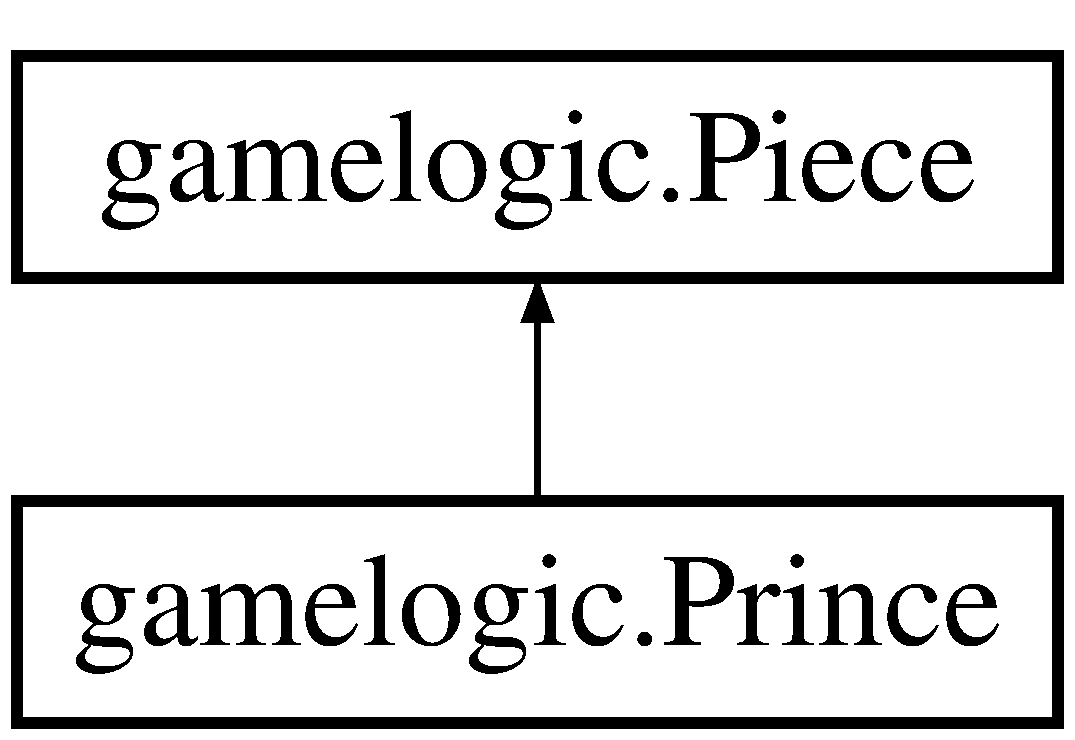
\includegraphics[height=2.000000cm]{classgamelogic_1_1_prince}
\end{center}
\end{figure}
\subsection*{Public Member Functions}
\begin{DoxyCompactItemize}
\item 
\mbox{\hyperlink{classgamelogic_1_1_prince_a7f45f9e01612930edfdaeb05a4f49f60}{Prince}} (\mbox{\hyperlink{classgamelogic_1_1_location}{Location}} location, \mbox{\hyperlink{classgamelogic_1_1_player}{Player}} player)
\item 
\mbox{\hyperlink{enumgamelogic_1_1_type}{Type}} \mbox{\hyperlink{classgamelogic_1_1_prince_aeb9994d7627fc4ff2e17844fefde51e3}{get\+Type}} ()
\item 
boolean \mbox{\hyperlink{classgamelogic_1_1_prince_a52427dfdfb25376c2435ada360e3a14c}{legal\+Movement}} (int toI, int toJ, \mbox{\hyperlink{classgamelogic_1_1_start}{Start}} start, \mbox{\hyperlink{classgamelogic_1_1_player}{Player}} player)
\end{DoxyCompactItemize}


\subsection{Constructor \& Destructor Documentation}
\mbox{\Hypertarget{classgamelogic_1_1_prince_a7f45f9e01612930edfdaeb05a4f49f60}\label{classgamelogic_1_1_prince_a7f45f9e01612930edfdaeb05a4f49f60}} 
\index{gamelogic\+::\+Prince@{gamelogic\+::\+Prince}!Prince@{Prince}}
\index{Prince@{Prince}!gamelogic\+::\+Prince@{gamelogic\+::\+Prince}}
\subsubsection{\texorpdfstring{Prince()}{Prince()}}
{\footnotesize\ttfamily gamelogic.\+Prince.\+Prince (\begin{DoxyParamCaption}\item[{\mbox{\hyperlink{classgamelogic_1_1_location}{Location}}}]{location,  }\item[{\mbox{\hyperlink{classgamelogic_1_1_player}{Player}}}]{player }\end{DoxyParamCaption})}

Constructor for \mbox{\hyperlink{classgamelogic_1_1_prince}{Prince}}. 
\begin{DoxyParams}{Parameters}
{\em board} & the board object of the current \mbox{\hyperlink{classgamelogic_1_1_board}{Board}} \\
\hline
{\em location} & the location object of the \mbox{\hyperlink{classgamelogic_1_1_board}{Board}} \\
\hline
{\em owner} & the Owner object associated with the \mbox{\hyperlink{classgamelogic_1_1_piece}{Piece}} \\
\hline
\end{DoxyParams}


\subsection{Member Function Documentation}
\mbox{\Hypertarget{classgamelogic_1_1_prince_aeb9994d7627fc4ff2e17844fefde51e3}\label{classgamelogic_1_1_prince_aeb9994d7627fc4ff2e17844fefde51e3}} 
\index{gamelogic\+::\+Prince@{gamelogic\+::\+Prince}!get\+Type@{get\+Type}}
\index{get\+Type@{get\+Type}!gamelogic\+::\+Prince@{gamelogic\+::\+Prince}}
\subsubsection{\texorpdfstring{get\+Type()}{getType()}}
{\footnotesize\ttfamily \mbox{\hyperlink{enumgamelogic_1_1_type}{Type}} gamelogic.\+Prince.\+get\+Type (\begin{DoxyParamCaption}{ }\end{DoxyParamCaption})}

A function that gets the \mbox{\hyperlink{classgamelogic_1_1_piece}{Piece}} type. \begin{DoxyReturn}{Returns}
an integer indicating the \mbox{\hyperlink{classgamelogic_1_1_piece}{Piece}} type 
\end{DoxyReturn}
\mbox{\Hypertarget{classgamelogic_1_1_prince_a52427dfdfb25376c2435ada360e3a14c}\label{classgamelogic_1_1_prince_a52427dfdfb25376c2435ada360e3a14c}} 
\index{gamelogic\+::\+Prince@{gamelogic\+::\+Prince}!legal\+Movement@{legal\+Movement}}
\index{legal\+Movement@{legal\+Movement}!gamelogic\+::\+Prince@{gamelogic\+::\+Prince}}
\subsubsection{\texorpdfstring{legal\+Movement()}{legalMovement()}}
{\footnotesize\ttfamily boolean gamelogic.\+Prince.\+legal\+Movement (\begin{DoxyParamCaption}\item[{int}]{toI,  }\item[{int}]{toJ,  }\item[{\mbox{\hyperlink{classgamelogic_1_1_start}{Start}}}]{start,  }\item[{\mbox{\hyperlink{classgamelogic_1_1_player}{Player}}}]{player }\end{DoxyParamCaption})}

check Validmove for \mbox{\hyperlink{classgamelogic_1_1_prince}{Prince}}. 
\begin{DoxyParams}{Parameters}
{\em x,designated} & row\textquotesingle{}s location \\
\hline
{\em y,designated} & col\textquotesingle{}s location \\
\hline
\end{DoxyParams}
\begin{DoxyReturn}{Returns}
boolean = true if it\textquotesingle{}s valid otherwise false 
\end{DoxyReturn}


The documentation for this class was generated from the following file\+:\begin{DoxyCompactItemize}
\item 
src/gamelogic/Prince.\+java\end{DoxyCompactItemize}

\hypertarget{classgamelogic_1_1_princess}{}\section{gamelogic.\+Princess Class Reference}
\label{classgamelogic_1_1_princess}\index{gamelogic.\+Princess@{gamelogic.\+Princess}}
Inheritance diagram for gamelogic.\+Princess\+:\begin{figure}[H]
\begin{center}
\leavevmode
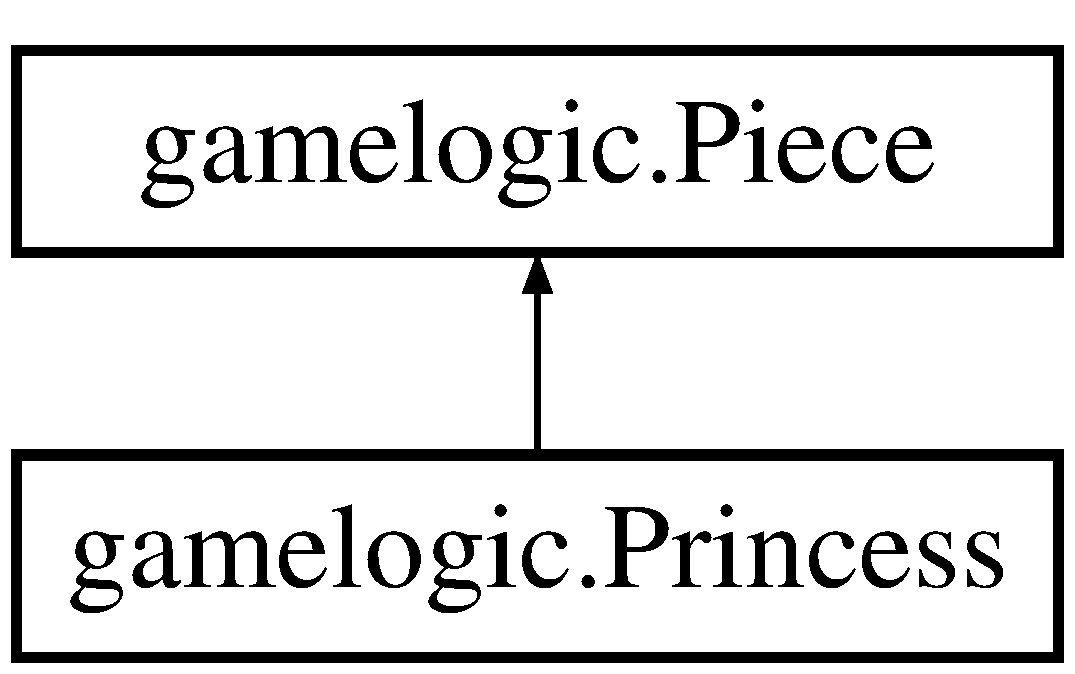
\includegraphics[height=2.000000cm]{classgamelogic_1_1_princess}
\end{center}
\end{figure}
\subsection*{Public Member Functions}
\begin{DoxyCompactItemize}
\item 
\mbox{\hyperlink{classgamelogic_1_1_princess_ac88224f446cffc47d38047cca0a8e6eb}{Princess}} (\mbox{\hyperlink{classgamelogic_1_1_location}{Location}} location, \mbox{\hyperlink{classgamelogic_1_1_player}{Player}} player)
\item 
\mbox{\hyperlink{enumgamelogic_1_1_type}{Type}} \mbox{\hyperlink{classgamelogic_1_1_princess_ad0792f772afda96bdc167331fdf139c5}{get\+Type}} ()
\item 
boolean \mbox{\hyperlink{classgamelogic_1_1_princess_a561f424db16e87b085990392ec151db4}{legal\+Movement}} (int toI, int toJ, \mbox{\hyperlink{classgamelogic_1_1_start}{Start}} start, \mbox{\hyperlink{classgamelogic_1_1_player}{Player}} player)
\end{DoxyCompactItemize}


\subsection{Constructor \& Destructor Documentation}
\mbox{\Hypertarget{classgamelogic_1_1_princess_ac88224f446cffc47d38047cca0a8e6eb}\label{classgamelogic_1_1_princess_ac88224f446cffc47d38047cca0a8e6eb}} 
\index{gamelogic\+::\+Princess@{gamelogic\+::\+Princess}!Princess@{Princess}}
\index{Princess@{Princess}!gamelogic\+::\+Princess@{gamelogic\+::\+Princess}}
\subsubsection{\texorpdfstring{Princess()}{Princess()}}
{\footnotesize\ttfamily gamelogic.\+Princess.\+Princess (\begin{DoxyParamCaption}\item[{\mbox{\hyperlink{classgamelogic_1_1_location}{Location}}}]{location,  }\item[{\mbox{\hyperlink{classgamelogic_1_1_player}{Player}}}]{player }\end{DoxyParamCaption})}

Constructor for \mbox{\hyperlink{classgamelogic_1_1_prince}{Prince}}. 
\begin{DoxyParams}{Parameters}
{\em board} & the board object of the current \mbox{\hyperlink{classgamelogic_1_1_board}{Board}} \\
\hline
{\em location} & the location object of the \mbox{\hyperlink{classgamelogic_1_1_board}{Board}} \\
\hline
{\em owner} & the Owner object associated with the \mbox{\hyperlink{classgamelogic_1_1_piece}{Piece}} \\
\hline
\end{DoxyParams}


\subsection{Member Function Documentation}
\mbox{\Hypertarget{classgamelogic_1_1_princess_ad0792f772afda96bdc167331fdf139c5}\label{classgamelogic_1_1_princess_ad0792f772afda96bdc167331fdf139c5}} 
\index{gamelogic\+::\+Princess@{gamelogic\+::\+Princess}!get\+Type@{get\+Type}}
\index{get\+Type@{get\+Type}!gamelogic\+::\+Princess@{gamelogic\+::\+Princess}}
\subsubsection{\texorpdfstring{get\+Type()}{getType()}}
{\footnotesize\ttfamily \mbox{\hyperlink{enumgamelogic_1_1_type}{Type}} gamelogic.\+Princess.\+get\+Type (\begin{DoxyParamCaption}{ }\end{DoxyParamCaption})}

A function that gets the \mbox{\hyperlink{classgamelogic_1_1_piece}{Piece}} type. \begin{DoxyReturn}{Returns}
an integer indicating the \mbox{\hyperlink{classgamelogic_1_1_piece}{Piece}} type 
\end{DoxyReturn}
\mbox{\Hypertarget{classgamelogic_1_1_princess_a561f424db16e87b085990392ec151db4}\label{classgamelogic_1_1_princess_a561f424db16e87b085990392ec151db4}} 
\index{gamelogic\+::\+Princess@{gamelogic\+::\+Princess}!legal\+Movement@{legal\+Movement}}
\index{legal\+Movement@{legal\+Movement}!gamelogic\+::\+Princess@{gamelogic\+::\+Princess}}
\subsubsection{\texorpdfstring{legal\+Movement()}{legalMovement()}}
{\footnotesize\ttfamily boolean gamelogic.\+Princess.\+legal\+Movement (\begin{DoxyParamCaption}\item[{int}]{toI,  }\item[{int}]{toJ,  }\item[{\mbox{\hyperlink{classgamelogic_1_1_start}{Start}}}]{start,  }\item[{\mbox{\hyperlink{classgamelogic_1_1_player}{Player}}}]{player }\end{DoxyParamCaption})}

check Validmove for \mbox{\hyperlink{classgamelogic_1_1_princess}{Princess}}. 
\begin{DoxyParams}{Parameters}
{\em x,designated} & row\textquotesingle{}s location \\
\hline
{\em y,designated} & col\textquotesingle{}s location \\
\hline
\end{DoxyParams}
\begin{DoxyReturn}{Returns}
boolean = true if it\textquotesingle{}s valid otherwise false 
\end{DoxyReturn}


The documentation for this class was generated from the following file\+:\begin{DoxyCompactItemize}
\item 
src/gamelogic/Princess.\+java\end{DoxyCompactItemize}

\hypertarget{class_tests_1_1_princess_test}{}\section{Tests.\+Princess\+Test Class Reference}
\label{class_tests_1_1_princess_test}\index{Tests.\+Princess\+Test@{Tests.\+Princess\+Test}}
\subsection*{Public Member Functions}
\begin{DoxyCompactItemize}
\item 
\mbox{\Hypertarget{class_tests_1_1_princess_test_a6137376a6c9cf152c577321aed3b226b}\label{class_tests_1_1_princess_test_a6137376a6c9cf152c577321aed3b226b}} 
void {\bfseries new\+Start} ()  throws Exception
\item 
\mbox{\Hypertarget{class_tests_1_1_princess_test_a8b8d640cd45ca2781f961e2a2773beac}\label{class_tests_1_1_princess_test_a8b8d640cd45ca2781f961e2a2773beac}} 
void {\bfseries valid\+Movements} ()
\item 
\mbox{\Hypertarget{class_tests_1_1_princess_test_a5685f4f37bb3c38bcb5cf581c3224f5f}\label{class_tests_1_1_princess_test_a5685f4f37bb3c38bcb5cf581c3224f5f}} 
void {\bfseries capture} ()  throws Exception 
\end{DoxyCompactItemize}


The documentation for this class was generated from the following file\+:\begin{DoxyCompactItemize}
\item 
src/\+Tests/Princess\+Test.\+java\end{DoxyCompactItemize}

\hypertarget{class_tests_1_1_prince_test}{}\section{Tests.\+Prince\+Test Class Reference}
\label{class_tests_1_1_prince_test}\index{Tests.\+Prince\+Test@{Tests.\+Prince\+Test}}
\subsection*{Public Member Functions}
\begin{DoxyCompactItemize}
\item 
\mbox{\Hypertarget{class_tests_1_1_prince_test_acddbc9b6d3180b184dff82127b9e825e}\label{class_tests_1_1_prince_test_acddbc9b6d3180b184dff82127b9e825e}} 
void {\bfseries new\+Start} ()  throws Exception
\item 
\mbox{\Hypertarget{class_tests_1_1_prince_test_a7b51e0bc503e990d07db7ae56fd89121}\label{class_tests_1_1_prince_test_a7b51e0bc503e990d07db7ae56fd89121}} 
void {\bfseries valid\+Movements} ()
\item 
\mbox{\Hypertarget{class_tests_1_1_prince_test_ab057f00ed482d5526e13c94faf61537d}\label{class_tests_1_1_prince_test_ab057f00ed482d5526e13c94faf61537d}} 
void {\bfseries capture} ()  throws Exception 
\end{DoxyCompactItemize}


The documentation for this class was generated from the following file\+:\begin{DoxyCompactItemize}
\item 
src/\+Tests/Prince\+Test.\+java\end{DoxyCompactItemize}

\hypertarget{classgamelogic_1_1_queen}{}\section{gamelogic.\+Queen Class Reference}
\label{classgamelogic_1_1_queen}\index{gamelogic.\+Queen@{gamelogic.\+Queen}}
Inheritance diagram for gamelogic.\+Queen\+:\begin{figure}[H]
\begin{center}
\leavevmode
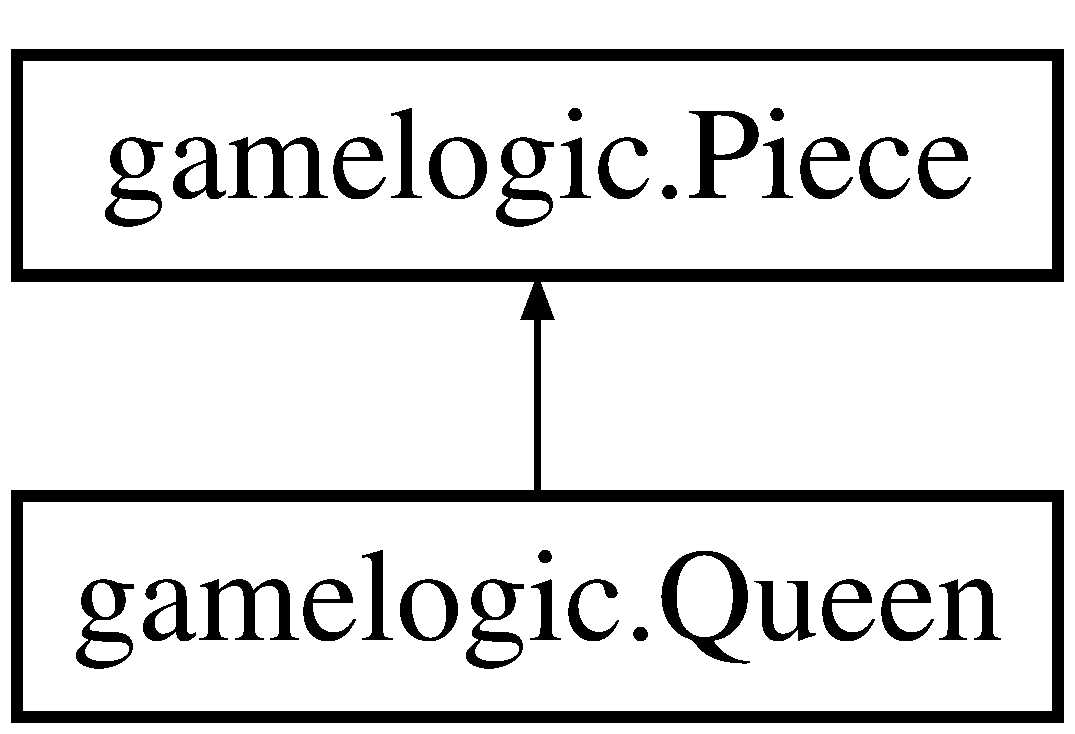
\includegraphics[height=2.000000cm]{classgamelogic_1_1_queen}
\end{center}
\end{figure}
\subsection*{Public Member Functions}
\begin{DoxyCompactItemize}
\item 
\mbox{\hyperlink{classgamelogic_1_1_queen_a2e4423ad97041b2638a6014c2743c83b}{Queen}} (\mbox{\hyperlink{classgamelogic_1_1_location}{Location}} location, \mbox{\hyperlink{classgamelogic_1_1_player}{Player}} player)
\item 
\mbox{\hyperlink{enumgamelogic_1_1_type}{Type}} \mbox{\hyperlink{classgamelogic_1_1_queen_af017112ee1d4b62e5a47c7874c063579}{get\+Type}} ()
\item 
boolean \mbox{\hyperlink{classgamelogic_1_1_queen_ad6d18289211705f1ab8e25b1daaba3a5}{legal\+Movement}} (int toI, int toJ, \mbox{\hyperlink{classgamelogic_1_1_start}{Start}} start, \mbox{\hyperlink{classgamelogic_1_1_player}{Player}} player)
\end{DoxyCompactItemize}


\subsection{Constructor \& Destructor Documentation}
\mbox{\Hypertarget{classgamelogic_1_1_queen_a2e4423ad97041b2638a6014c2743c83b}\label{classgamelogic_1_1_queen_a2e4423ad97041b2638a6014c2743c83b}} 
\index{gamelogic\+::\+Queen@{gamelogic\+::\+Queen}!Queen@{Queen}}
\index{Queen@{Queen}!gamelogic\+::\+Queen@{gamelogic\+::\+Queen}}
\subsubsection{\texorpdfstring{Queen()}{Queen()}}
{\footnotesize\ttfamily gamelogic.\+Queen.\+Queen (\begin{DoxyParamCaption}\item[{\mbox{\hyperlink{classgamelogic_1_1_location}{Location}}}]{location,  }\item[{\mbox{\hyperlink{classgamelogic_1_1_player}{Player}}}]{player }\end{DoxyParamCaption})}

Constructor for \mbox{\hyperlink{classgamelogic_1_1_queen}{Queen}}. 
\begin{DoxyParams}{Parameters}
{\em board} & the board object of the current \mbox{\hyperlink{classgamelogic_1_1_board}{Board}} \\
\hline
{\em location} & the location object of the \mbox{\hyperlink{classgamelogic_1_1_board}{Board}} \\
\hline
{\em owner} & the Owner object associated with the \mbox{\hyperlink{classgamelogic_1_1_piece}{Piece}} \\
\hline
\end{DoxyParams}


\subsection{Member Function Documentation}
\mbox{\Hypertarget{classgamelogic_1_1_queen_af017112ee1d4b62e5a47c7874c063579}\label{classgamelogic_1_1_queen_af017112ee1d4b62e5a47c7874c063579}} 
\index{gamelogic\+::\+Queen@{gamelogic\+::\+Queen}!get\+Type@{get\+Type}}
\index{get\+Type@{get\+Type}!gamelogic\+::\+Queen@{gamelogic\+::\+Queen}}
\subsubsection{\texorpdfstring{get\+Type()}{getType()}}
{\footnotesize\ttfamily \mbox{\hyperlink{enumgamelogic_1_1_type}{Type}} gamelogic.\+Queen.\+get\+Type (\begin{DoxyParamCaption}{ }\end{DoxyParamCaption})}

A function that gets the \mbox{\hyperlink{classgamelogic_1_1_piece}{Piece}} type. \begin{DoxyReturn}{Returns}
an integer indicating the \mbox{\hyperlink{classgamelogic_1_1_piece}{Piece}} type 
\end{DoxyReturn}
\mbox{\Hypertarget{classgamelogic_1_1_queen_ad6d18289211705f1ab8e25b1daaba3a5}\label{classgamelogic_1_1_queen_ad6d18289211705f1ab8e25b1daaba3a5}} 
\index{gamelogic\+::\+Queen@{gamelogic\+::\+Queen}!legal\+Movement@{legal\+Movement}}
\index{legal\+Movement@{legal\+Movement}!gamelogic\+::\+Queen@{gamelogic\+::\+Queen}}
\subsubsection{\texorpdfstring{legal\+Movement()}{legalMovement()}}
{\footnotesize\ttfamily boolean gamelogic.\+Queen.\+legal\+Movement (\begin{DoxyParamCaption}\item[{int}]{toI,  }\item[{int}]{toJ,  }\item[{\mbox{\hyperlink{classgamelogic_1_1_start}{Start}}}]{start,  }\item[{\mbox{\hyperlink{classgamelogic_1_1_player}{Player}}}]{player }\end{DoxyParamCaption})}

check Validmove for \mbox{\hyperlink{classgamelogic_1_1_queen}{Queen}}. 
\begin{DoxyParams}{Parameters}
{\em toX,designated} & row\textquotesingle{}s location \\
\hline
{\em toY,designated} & col\textquotesingle{}s location \\
\hline
\end{DoxyParams}
\begin{DoxyReturn}{Returns}
boolean = true if it\textquotesingle{}s valid otherwise false 
\end{DoxyReturn}


The documentation for this class was generated from the following file\+:\begin{DoxyCompactItemize}
\item 
src/gamelogic/Queen.\+java\end{DoxyCompactItemize}

\hypertarget{class_tests_1_1_queen_test}{}\section{Tests.\+Queen\+Test Class Reference}
\label{class_tests_1_1_queen_test}\index{Tests.\+Queen\+Test@{Tests.\+Queen\+Test}}
\subsection*{Public Member Functions}
\begin{DoxyCompactItemize}
\item 
\mbox{\Hypertarget{class_tests_1_1_queen_test_a8bd69332b6be70d7f76ed7c818f2887b}\label{class_tests_1_1_queen_test_a8bd69332b6be70d7f76ed7c818f2887b}} 
void {\bfseries new\+Start} ()  throws Exception
\item 
\mbox{\Hypertarget{class_tests_1_1_queen_test_ad7441261fb59635664b6db2219ce7ebd}\label{class_tests_1_1_queen_test_ad7441261fb59635664b6db2219ce7ebd}} 
void {\bfseries valid\+Movements} ()
\item 
\mbox{\Hypertarget{class_tests_1_1_queen_test_a8ee094e0194b63141e22a505f7883592}\label{class_tests_1_1_queen_test_a8ee094e0194b63141e22a505f7883592}} 
void {\bfseries valid\+Movements\+Up} ()
\item 
\mbox{\Hypertarget{class_tests_1_1_queen_test_aed4049e484d9eb959ff6542548f2b1f1}\label{class_tests_1_1_queen_test_aed4049e484d9eb959ff6542548f2b1f1}} 
void {\bfseries valid\+Movements\+Down} ()
\item 
\mbox{\Hypertarget{class_tests_1_1_queen_test_aa4037ca413dde45e855c193e7dc1db30}\label{class_tests_1_1_queen_test_aa4037ca413dde45e855c193e7dc1db30}} 
void {\bfseries capture} ()  throws Exception 
\end{DoxyCompactItemize}


The documentation for this class was generated from the following file\+:\begin{DoxyCompactItemize}
\item 
src/\+Tests/Queen\+Test.\+java\end{DoxyCompactItemize}

\hypertarget{classgamelogic_1_1_rook}{}\section{gamelogic.\+Rook Class Reference}
\label{classgamelogic_1_1_rook}\index{gamelogic.\+Rook@{gamelogic.\+Rook}}
Inheritance diagram for gamelogic.\+Rook\+:\begin{figure}[H]
\begin{center}
\leavevmode
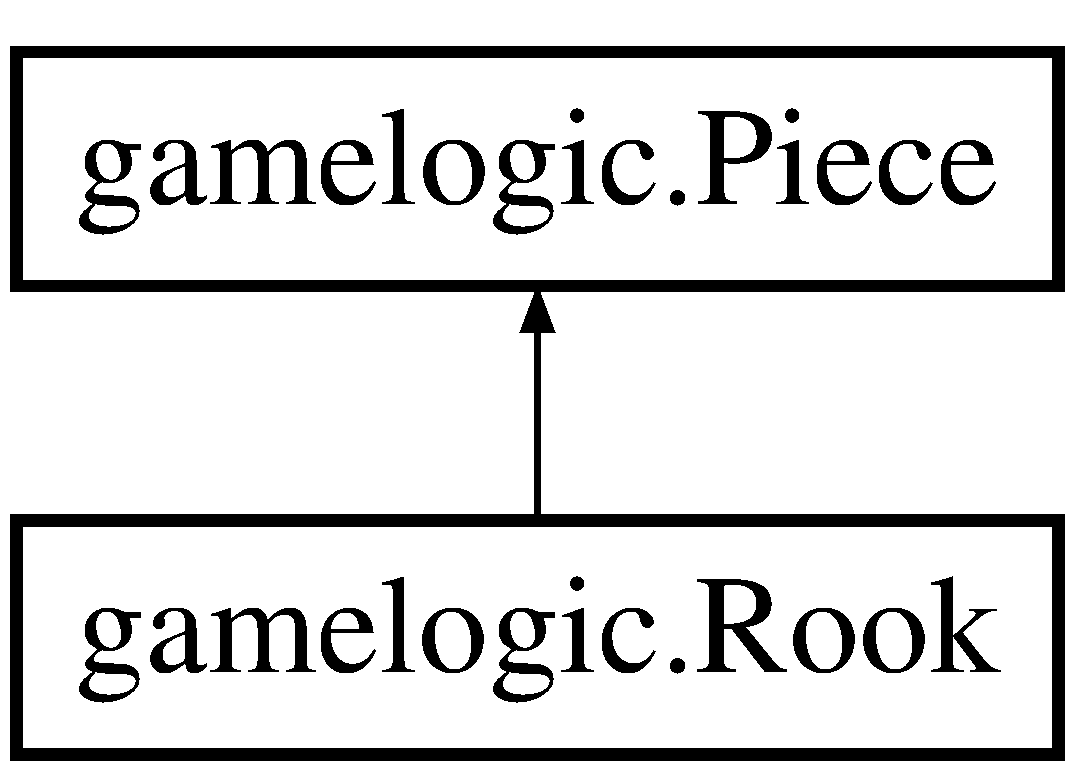
\includegraphics[height=2.000000cm]{classgamelogic_1_1_rook}
\end{center}
\end{figure}
\subsection*{Public Member Functions}
\begin{DoxyCompactItemize}
\item 
\mbox{\hyperlink{classgamelogic_1_1_rook_aa326432823f48a6a727ec4df70d28849}{Rook}} (\mbox{\hyperlink{classgamelogic_1_1_location}{Location}} location, \mbox{\hyperlink{classgamelogic_1_1_player}{Player}} player)
\item 
\mbox{\hyperlink{enumgamelogic_1_1_type}{Type}} \mbox{\hyperlink{classgamelogic_1_1_rook_a65532b2680c7e661be8aff40304fbeef}{get\+Type}} ()
\item 
boolean \mbox{\hyperlink{classgamelogic_1_1_rook_a655f65fd697faa14fb21952167157621}{legal\+Movement}} (int toI, int toJ, \mbox{\hyperlink{classgamelogic_1_1_start}{Start}} start, \mbox{\hyperlink{classgamelogic_1_1_player}{Player}} player)
\end{DoxyCompactItemize}


\subsection{Constructor \& Destructor Documentation}
\mbox{\Hypertarget{classgamelogic_1_1_rook_aa326432823f48a6a727ec4df70d28849}\label{classgamelogic_1_1_rook_aa326432823f48a6a727ec4df70d28849}} 
\index{gamelogic\+::\+Rook@{gamelogic\+::\+Rook}!Rook@{Rook}}
\index{Rook@{Rook}!gamelogic\+::\+Rook@{gamelogic\+::\+Rook}}
\subsubsection{\texorpdfstring{Rook()}{Rook()}}
{\footnotesize\ttfamily gamelogic.\+Rook.\+Rook (\begin{DoxyParamCaption}\item[{\mbox{\hyperlink{classgamelogic_1_1_location}{Location}}}]{location,  }\item[{\mbox{\hyperlink{classgamelogic_1_1_player}{Player}}}]{player }\end{DoxyParamCaption})}

Constructor for \mbox{\hyperlink{classgamelogic_1_1_rook}{Rook}}. 
\begin{DoxyParams}{Parameters}
{\em board} & the board object of the current \mbox{\hyperlink{classgamelogic_1_1_board}{Board}} \\
\hline
{\em location} & the location object of the \mbox{\hyperlink{classgamelogic_1_1_board}{Board}} \\
\hline
{\em owner} & the Owner object associated with the \mbox{\hyperlink{classgamelogic_1_1_piece}{Piece}} \\
\hline
\end{DoxyParams}


\subsection{Member Function Documentation}
\mbox{\Hypertarget{classgamelogic_1_1_rook_a65532b2680c7e661be8aff40304fbeef}\label{classgamelogic_1_1_rook_a65532b2680c7e661be8aff40304fbeef}} 
\index{gamelogic\+::\+Rook@{gamelogic\+::\+Rook}!get\+Type@{get\+Type}}
\index{get\+Type@{get\+Type}!gamelogic\+::\+Rook@{gamelogic\+::\+Rook}}
\subsubsection{\texorpdfstring{get\+Type()}{getType()}}
{\footnotesize\ttfamily \mbox{\hyperlink{enumgamelogic_1_1_type}{Type}} gamelogic.\+Rook.\+get\+Type (\begin{DoxyParamCaption}{ }\end{DoxyParamCaption})}

A function that gets the \mbox{\hyperlink{classgamelogic_1_1_piece}{Piece}} type. \begin{DoxyReturn}{Returns}
an integer indicating the \mbox{\hyperlink{classgamelogic_1_1_piece}{Piece}} type 
\end{DoxyReturn}
\mbox{\Hypertarget{classgamelogic_1_1_rook_a655f65fd697faa14fb21952167157621}\label{classgamelogic_1_1_rook_a655f65fd697faa14fb21952167157621}} 
\index{gamelogic\+::\+Rook@{gamelogic\+::\+Rook}!legal\+Movement@{legal\+Movement}}
\index{legal\+Movement@{legal\+Movement}!gamelogic\+::\+Rook@{gamelogic\+::\+Rook}}
\subsubsection{\texorpdfstring{legal\+Movement()}{legalMovement()}}
{\footnotesize\ttfamily boolean gamelogic.\+Rook.\+legal\+Movement (\begin{DoxyParamCaption}\item[{int}]{toI,  }\item[{int}]{toJ,  }\item[{\mbox{\hyperlink{classgamelogic_1_1_start}{Start}}}]{start,  }\item[{\mbox{\hyperlink{classgamelogic_1_1_player}{Player}}}]{player }\end{DoxyParamCaption})}

check Validmove for \mbox{\hyperlink{classgamelogic_1_1_rook}{Rook}}. 
\begin{DoxyParams}{Parameters}
{\em x,designated} & row\textquotesingle{}s location \\
\hline
{\em y,designated} & col\textquotesingle{}s location \\
\hline
\end{DoxyParams}
\begin{DoxyReturn}{Returns}
boolean = true if it\textquotesingle{}s valid otherwise false 
\end{DoxyReturn}


The documentation for this class was generated from the following file\+:\begin{DoxyCompactItemize}
\item 
src/gamelogic/Rook.\+java\end{DoxyCompactItemize}

\hypertarget{class_tests_1_1_rook_test}{}\section{Tests.\+Rook\+Test Class Reference}
\label{class_tests_1_1_rook_test}\index{Tests.\+Rook\+Test@{Tests.\+Rook\+Test}}
\subsection*{Public Member Functions}
\begin{DoxyCompactItemize}
\item 
\mbox{\Hypertarget{class_tests_1_1_rook_test_aa0689fccf73fbb78214f6685cca09687}\label{class_tests_1_1_rook_test_aa0689fccf73fbb78214f6685cca09687}} 
void {\bfseries new\+Start} ()  throws Exception
\item 
\mbox{\Hypertarget{class_tests_1_1_rook_test_a14906a143a65e096bc060716325b06a9}\label{class_tests_1_1_rook_test_a14906a143a65e096bc060716325b06a9}} 
void {\bfseries valid\+Movements\+Right} ()
\item 
\mbox{\Hypertarget{class_tests_1_1_rook_test_a1b97b4ac991136ca0d616e9a7224381e}\label{class_tests_1_1_rook_test_a1b97b4ac991136ca0d616e9a7224381e}} 
void {\bfseries valid\+Movements\+Up} ()
\item 
\mbox{\Hypertarget{class_tests_1_1_rook_test_aefff3f4e857073c54c97cb04a0248dc5}\label{class_tests_1_1_rook_test_aefff3f4e857073c54c97cb04a0248dc5}} 
void {\bfseries invalid\+Movements\+Diagonal} ()
\item 
\mbox{\Hypertarget{class_tests_1_1_rook_test_a1a12e20c64eeb9c5f2d3e4fc5e8bb45c}\label{class_tests_1_1_rook_test_a1a12e20c64eeb9c5f2d3e4fc5e8bb45c}} 
void {\bfseries capture\+Pieces} ()  throws Exception 
\end{DoxyCompactItemize}


The documentation for this class was generated from the following file\+:\begin{DoxyCompactItemize}
\item 
src/\+Tests/Rook\+Test.\+java\end{DoxyCompactItemize}

\hypertarget{classgamelogic_1_1_start}{}\section{gamelogic.\+Start Class Reference}
\label{classgamelogic_1_1_start}\index{gamelogic.\+Start@{gamelogic.\+Start}}
\subsection*{Public Member Functions}
\begin{DoxyCompactItemize}
\item 
\mbox{\Hypertarget{classgamelogic_1_1_start_a161eefcd26dc8dce8a27a8b73f1285b4}\label{classgamelogic_1_1_start_a161eefcd26dc8dce8a27a8b73f1285b4}} 
void {\bfseries set\+New\+Game} ()
\item 
\mbox{\Hypertarget{classgamelogic_1_1_start_adc13d7ee88e45fc4a76192358521c88d}\label{classgamelogic_1_1_start_adc13d7ee88e45fc4a76192358521c88d}} 
\mbox{\hyperlink{classgamelogic_1_1_board}{Board}} {\bfseries get\+Board} ()
\end{DoxyCompactItemize}
\subsection*{Public Attributes}
\begin{DoxyCompactItemize}
\item 
\mbox{\Hypertarget{classgamelogic_1_1_start_a2ac837ad7b528d4a29aa72917a46c654}\label{classgamelogic_1_1_start_a2ac837ad7b528d4a29aa72917a46c654}} 
\mbox{\hyperlink{classgamelogic_1_1_board}{Board}} {\bfseries board}
\item 
\mbox{\Hypertarget{classgamelogic_1_1_start_aaab56a58607a3cb8d8e326c3c475fa0e}\label{classgamelogic_1_1_start_aaab56a58607a3cb8d8e326c3c475fa0e}} 
\mbox{\hyperlink{classgamelogic_1_1_player}{Player}} {\bfseries player\+White}
\end{DoxyCompactItemize}


The documentation for this class was generated from the following file\+:\begin{DoxyCompactItemize}
\item 
src/gamelogic/Start.\+java\end{DoxyCompactItemize}

\hypertarget{class_gui_1_1_table}{}\section{Gui.\+Table Class Reference}
\label{class_gui_1_1_table}\index{Gui.\+Table@{Gui.\+Table}}
\subsection*{Static Public Member Functions}
\begin{DoxyCompactItemize}
\item 
\mbox{\Hypertarget{class_gui_1_1_table_aa3ea31ce1a22749e70a7256a7996ef97}\label{class_gui_1_1_table_aa3ea31ce1a22749e70a7256a7996ef97}} 
static void {\bfseries main} (String\mbox{[}$\,$\mbox{]} args)
\end{DoxyCompactItemize}


The documentation for this class was generated from the following file\+:\begin{DoxyCompactItemize}
\item 
src/\+Gui/Table.\+java\end{DoxyCompactItemize}

\hypertarget{enumgamelogic_1_1_type}{}\section{gamelogic.\+Type Enum Reference}
\label{enumgamelogic_1_1_type}\index{gamelogic.\+Type@{gamelogic.\+Type}}
\subsection*{Public Attributes}
\begin{DoxyCompactItemize}
\item 
\mbox{\Hypertarget{enumgamelogic_1_1_type_abf0533404306835768de03bbbe47cbfd}\label{enumgamelogic_1_1_type_abf0533404306835768de03bbbe47cbfd}} 
{\bfseries K\+N\+I\+G\+HT}
\item 
\mbox{\Hypertarget{enumgamelogic_1_1_type_a456bda7e831b59ee1008a5121b1a6ab8}\label{enumgamelogic_1_1_type_a456bda7e831b59ee1008a5121b1a6ab8}} 
{\bfseries K\+I\+NG}
\item 
\mbox{\Hypertarget{enumgamelogic_1_1_type_a5b6ab48650f63932b9be133afe0e266d}\label{enumgamelogic_1_1_type_a5b6ab48650f63932b9be133afe0e266d}} 
{\bfseries R\+O\+OK}
\item 
\mbox{\Hypertarget{enumgamelogic_1_1_type_a12ed260808e761ee21e6aa29f2154915}\label{enumgamelogic_1_1_type_a12ed260808e761ee21e6aa29f2154915}} 
{\bfseries P\+A\+WN}
\item 
\mbox{\Hypertarget{enumgamelogic_1_1_type_a6da8ee06cce75fa08f0a984ef7e84f42}\label{enumgamelogic_1_1_type_a6da8ee06cce75fa08f0a984ef7e84f42}} 
{\bfseries B\+I\+S\+H\+OP}
\item 
\mbox{\Hypertarget{enumgamelogic_1_1_type_a2e9397920ba6abf38cc942de8a484fcb}\label{enumgamelogic_1_1_type_a2e9397920ba6abf38cc942de8a484fcb}} 
{\bfseries Q\+U\+E\+EN}
\item 
\mbox{\Hypertarget{enumgamelogic_1_1_type_abd4398549d5aee3ba9444d5ac92161ca}\label{enumgamelogic_1_1_type_abd4398549d5aee3ba9444d5ac92161ca}} 
{\bfseries P\+R\+I\+N\+CE}
\item 
\mbox{\Hypertarget{enumgamelogic_1_1_type_a969c8cc9de737587a1d6237e43b6ac13}\label{enumgamelogic_1_1_type_a969c8cc9de737587a1d6237e43b6ac13}} 
{\bfseries P\+R\+I\+N\+C\+E\+SS}
\end{DoxyCompactItemize}


The documentation for this enum was generated from the following file\+:\begin{DoxyCompactItemize}
\item 
src/gamelogic/Type.\+java\end{DoxyCompactItemize}

%--- End generated contents ---

% Index
\backmatter
\newpage
\phantomsection
\clearemptydoublepage
\addcontentsline{toc}{chapter}{Index}
\printindex

\end{document}
